\documentclass[12pt]{uthesis-v12}  %---> DO NOT ALTER THIS COMMAND

\usepackage{hyperref}
\usepackage{epigraph}
\usepackage{listings}

\usepackage[dvips]{graphicx}
\graphicspath{{images/}}
\DeclareGraphicsExtensions{.eps}


\begin{document} %---> %---> %---> %---> DO NOT ALTER THIS COMMAND

%--------+----------------------------------------------------------+
%        |  \title{}                                    (REQUIRED)  |
%        |  \author{}                                   (REQUIRED)  |
%        |                                                          |
%        |  See section 3.1 of "Read_Me_First_(v12).pdf"            |
%        |                                                          |
%        |  Also see section 2.2 of above "Read Me" file for the    |
%        |  proper use of the invisible tilde ("~") character when  |
%        |  entering a middle initial in the \author command.       |
%        +----------------------------------------------------------+

\title{combox}

\author{Siddharth Ravikumar}

%--------+----------------------------------------------------------+
%        |  \copyrightpage{}                            (REQUIRED)  |
%        |                                                          |
%        |  See section 3.2 of "Read_Me_First_(v12).pdf"            |
%        |                                                          |
%        |  1) You must enter either "yes" or "no" in this          |
%        |      command.  Inputting "yes" produces a copyright      |
%        |      notification page as the second page and inputting  |
%        |      "no" produces a blank second page.                  |
%        |  2) Input to this command is case sensitive.             |
%        |  3) Default: the "yes" option.                           |
%        +----------------------------------------------------------+

\copyrightpage{yes}

%--------+----------------------------------------------------------+
%        |  \mydocument{}                               (REQUIRED)  |
%        |                                                          |
%        |  See section 3.3 of "Read_Me_First_(v12).pdf"            |
%        |                                                          |
%        |  1) Input to this command is limited to the following    |
%        |     three options: a) Dissertation                       |
%        |                    b) Thesis                             |
%        |                    c) Project                            |
%        |  2) Input to this command is case-sensitive.             |
%        +----------------------------------------------------------+

\mydocument{Project}

%--------+----------------------------------------------------------+
%        |  \degree{}{}                                 (REQUIRED)  |
%        |                                                          |
%        |  See section 3.4 of "Read_Me_First_(v12).pdf"            |
%        |                                                          |
%        |  You need to provide two distinct inputs into this       |
%        |  command:                                                |
%        |     1) In the first set of braces you need to specify    |
%        |        the *exact* degree you will receive. Some         |
%        |        examples are: -) Masters of Arts                  |
%        |                      -) Masters of Science               |
%        |                      -) Doctor of Philosophy             |
%        |     2) In the second set of braces you need to state the |
%        |        *specific* discipline or area for that degree     |
%        |        (e.g., Economics, Education, Engineering, etc.).  |
%        |  Students should consult their advisor if they have any  |
%        |  questions about this information.                       |
%        +----------------------------------------------------------+

\degree{Masters of Science}{Computer Science}

%--------+----------------------------------------------------------+
%        |  \conferraldate{}{}                          (REQUIRED)  |
%        |                                                          |
%        |  See section 3.5 of "Read_Me_First_(v12).pdf"            |
%        |                                                          |
%        |  In the two set of braces enter the month and then the   |
%        |  year your degree will be *conferred* by the university. |
%        +----------------------------------------------------------+

\conferraldate{May}{2016}

%--------+----------------------------------------------------------+
%        |  \advisor{}                                  (REQUIRED)  |
%        |                                                          |
%        |  See section 3.6.2 of "Read_Me_First_(v12).pdf"          |
%        |                                                          |
%        |  1) Also see section 2.2 of "Read_Me_First_(v12).pdf"    |
%        |     for the proper use of the invisible tilde ("~")      |
%        |     character when entering a middle initial or the      |
%        |     abbreviation of an academic title (e.g., Dr.) in     |
%        |     the \advisor{} command.                              |
%        |  2) Also see section 3.6.1. for consistent presentation  |
%        |     of title page signature lines.                       |
%        +----------------------------------------------------------+

\advisor{Dr.~Robert C. Green II}

%--------+----------------------------------------------------------+
%        |  Committee Member Signature Commands         (OPTIONAL)  |
%        |                                                          |
%        |  See section 3.6.3 of "Read_Me_First_(v12).pdf"          |
%        |                                                          |
%        |  1) Use the commands below to provide signature lines    |
%        |     for your "other" committee members;                  |
%        |        --> you must list your other committee members    |
%        |            in alphabetic order by last name              |
%        |        --> to do this, use the commands below in the     |
%        |            order presented below.                        |
%        |  2) You can choose to include none, some, or all of the  |
%        |     "XXXmember" commands below --- based on the number   |
%        |     committee members you have; simply delete (or        |
%        |     comment-out) any of the commands below that are not  |
%        |     needed.                                              |
%        |  3) Do not include the name of your committee chair or   |
%        |     the Graduate Dean in the commands listed below.      |
%        |     Their signature lines are generated by the           |
%        |     \advisor{} and \graduatedean{}{} commands.           |
%        |  4) You cannot use any of the commands below more than   |
%        |     once. (For details on this issue, see section 3.6.3  |
%        |     of "Read_Me_First_(v12).pdf".)                       |
%        |  5) Also see section 2.2 of "Read_Me_First_(v12).pdf"    |
%        |     for the proper use of the invisible tilde ("~")      |
%        |     character when entering a middle initial or the      |
%        |     abbreviation of an academic title (e.g., Dr.) in     |
%        |     the commands below.                                  |
%        |  6) See section 3.6.1. for consistent presentation of    |
%        |     title page signature lines.                          |
%        |                                                          |
%        |  I know I shouldn't have to say this, but enough         |
%        |  students over the years have made the same mistake      |
%        |  that I'm forced to state:                               |
%        |                                                          |
%        |      THE NAMES USED IN THE FOLLOWING COMMANDS ARE        |
%        |      SILLY NAMES I'VE USED AS EXAMPLES ONLY.  THEY       |
%        |      ARE NOT THE ACTUAL NAMES OF YOUR COMMITTEE          |
%        |      MEMBERS.  REPLACE THE SILLY NAMES BELOW WITH        |
%        |      THE NAMES OF YOUR ACTUAL COMMITTEE MEMBERS.         |
%        |                                                          |
%        +----------------------------------------------------------+

%--------+----------------------------------------------------------+
%        |  \graduatedean{}{}                           (REQUIRED)  |
%        |                                                          |
%        |  See section 3.6.4 of "Read_Me_First_(v12).pdf"          |
%        |                                                          |
%        |  1) THE NAME AND TITLE PROVIDED BELOW ARE THOSE OF THE   |
%        |     ACTUAL GRADUATE DEAN AT THE TIME THIS DOCUMENT WAS   |
%        |     CONSTRUCTED (January 2012). Contact the Graduate     |
%        |     College to determine whether this information is     |
%        |     correct at the time you submit your document.        |
%        |  2) Section 2.2 of "Read_Me_First_(v12).pdf" describes   |
%        |     the proper use of the invisible tilde ("~")          |
%        |     character when entering a middle initial or the      |
%        |     abbreviation of an academic title (e.g., Dr.) in     |
%        |     the \graduatedean{} command.                         |
%        |  3) See section 3.6.1. for consistent presentation of    |
%        |     title page signature lines.                          |
%        +----------------------------------------------------------+

\graduatedean{Dr.~Michael Ogawa}{Dean}

%--------+----------------------------------------------------------+
%        |  \maketitle                                  (REQUIRED)  |
%        |                                                          |
%        |  See section 3.7 of "Read_Me_First_(v12).pdf"            |
%        |                                                          |
%        |  This is a required LaTeX command; to be brief, bad      |
%        |  things will happen if this command is not included      |
%        |  in your document at this particular location.           |
%        +----------------------------------------------------------+

\maketitle  %---->  ----->  ---->  ---->   DO NOT ALTER THIS COMMAND

%--------+----------------------------------------------------------+
%        |  Abstract Page Environment                   (REQUIRED)  |
%        |                                                          |
%        |  See section 3.8 of "Read_Me_First_(v12).pdf"            |
%        +----------------------------------------------------------+

%--------+----------------------------------------------------------+
%        |  Dedication Page Environment                 (OPTIONAL)  |
%        |                                                          |
%        |  See section 3.9 of "Read_Me_First_(v12).pdf"            |
%        |                                                          |
%        |  If both a dedication page and an acknowledgements page  |
%        |  are included in the document, the dedication page must  |
%        |  proceed the acknowledgements page.                      |
%        +----------------------------------------------------------+

% abstract
\begin{abstractpage}\label{combox-abstract}
  File storage providers on the Internet have made it non-trivial for
  individuals to store their personal files online. At the same time,
  there has been revelations about the existence of a billion dollar
  surveillance industry\cite{website:wikileaks-spyfiles} that is
  building and selling tools to governments and dictatorships to snoop
  on its own citizens. In a world which is fast becoming Orwellian,
  storing personal files on storage provided by file storage providers
  is not even an option for some individuals. In the past, there have
  been separate efforts to come up with a solution to allow
  individuals to use storage space provided by file storage providers
  in a way that it made it impossible for file storage providers or
  ``third parties'' to access the user' files. combox is one such
  effort, it allows an individual to store their personal files on the
  storage provided by Google Drive and Dropbox in such a way that only
  part of each file (in encrypted form) is stored in Google
  Drive/Dropbox. combox is a python package compatible with GNU/Linux
  and OS X platforms. This report contains an overview of combox --
  what it is, how it was developed and tested; explains how combox is
  different from Vollmar's Combo-Box\cite{vollmar-combo-box}; reviews
  projects similar to combox that help computer users to securely
  store personal files on storage provided by file storage providers;
  lastly, enlists things that can be done to improve combox.
\end{abstractpage}


%--------+----------------------------------------------------------+
%        |  Acknowledgments Page Environment            (OPTIONAL)  |
%        |                                                          |
%        |  See section 3.10 of "Read_Me_First_(v12).pdf"           |
%        |                                                          |
%        |  If both a dedication page and an acknowledgements page  |
%        |  are included in the document, the dedication page must  |
%        |  proceed the acknowledgements page.                      |
%        +----------------------------------------------------------+
% dedication
\begin{dedication}
  \noindent Dedicated to the
  \verb+$EDITOR+ I use to literally write everything.
\end{dedication}

%--------+----------------------------------------------------------+
%        |  \tableofcontents                            (REQUIRED)  |
%        |  \listoftables                            (CONDITIONAL)  |
%        |  \listoffigures                           (CONDITIONAL)  |
%        |                                                          |
%        |  See sections 3.11 & 3.12 of "Read_Me_First_(v12).pdf"   |
%        |                                                          |
%        |  1) You must include the \tableofcontents command in     |
%        |     your document: the UT Manual requires every          |
%        |     dissertation/thesis to have a detailed table of      |
%        |     contents.                                            |
%        |  2) Including the \listoftables and \listoffigures       |
%        |     commands is "conditional."  See sections 3.12 of     |
%        |     "Read_Me_First_(v12).pdf" for additional details.    |
%        +----------------------------------------------------------+
% acknowledgments
% Public Domain. No Rights Reserved. See
% https://creativecommons.org/publicdomain/zero/1.0/

\section*{Acknowledgments}

\begin{frame}
  \frametitle{Acknowledgments}
  Dr. Robert C. Green II
\end{frame}

\tableofcontents  %----->  ----->  ---->  DO NOT ALTER THIS COMMAND
\listoftables \listoffigures

%--------+----------------------------------------------------------+
%        |  \captionformat{}                            (REQUIRED)  |
%        |                                                          |
%        |  See section 3.12.2 of "Read_Me_First_(v12).pdf"         |
%        |                                                          |
%        |  1) You are required to choose between the "hang" or     |
%        |     "align" option for this command.                     |
%        |  2) Input to this command is case sensitive.             |
%        |  3) Default: ``hang'' option.                            |
%        +----------------------------------------------------------+

\captionformat{hang}

%--------+----------------------------------------------------------+
%        |  List of Abbreviations Environment           (OPTIONAL)  |
%        |                                                          |
%        |  See section 3.13 of "Read_Me_First_(v12).pdf"           |
%        |                                                          |
%        |  1) This is an optional section; consult your advisor    |
%        |     to determine whether you need/want to include this   |
%        |     section in your document.                            |
%        |  2) If you do not want a List of Abbreviations simply    |
%        |     delete the material below (and these instructions).  |
%        |  3) If you do want a List of Abbreviations simply        |
%        |     replace the silly material below with the            |
%        |     information relevant to your document.               |
%        |     a. Within the "listofabbreviations" environment      |
%        |        below you must use a separate \abbreviation{}{}   |
%        |        command for each entry in your List of            |
%        |        Abbreviations.                                    |
%        |     b. As the examples below demonstrate, the            |
%        |        information within the first set of braces is     |
%        |        the abbreviation and the information in the       |
%        |        second set of braces is the definition of that    |
%        |        abbreviation.                                     |
%        +----------------------------------------------------------+

\begin{listofabbreviations}

    \abbreviation{YAML}{YAML Ain't Markup Language}
    \abbreviation{CLI}{Command Line Interface}
    \abbreviation{GUI}{Graphical User Interface}
    \abbreviation{JSON}{JavaScript Object Notation}

\end{listofabbreviations}



%--------+----------------------------------------------------------+
%        |  Preface Environment                         (OPTIONAL)  |
%        |                                                          |
%        |  See section 3.15 of "Read_Me_First_(v12).pdf"           |
%        +----------------------------------------------------------+


%XXXXXXXXXXXXXXXXXXXXXXXXXXXXXXXXXXXXXXXXXXXXXXXXXXXXXXXXXXXXXXXXXXXX
%XXXXXXXXXXXXXXXXXXXXXXXXXXXXXXXXXXXXXXXXXXXXXXXXXXXXXXXXXXXXXXXXXXXX
%XXXXXXXXXXXXXXXXXXXXXXXXXXXXXXXXXXXXXXXXXXXXXXXXXXXXXXXXXXXXXXXXXXXX
%XXXXXXXXXXXXXXXXXXXXXXXXXXXXXXXXXXXXXXXXXXXXXXXXXXXXXXXXXXXXXXXXXXXX
\begin{preface}
 Faithfully follow the steps below with utmost diligence; begin reading step 1.

 \begin{enumerate}
   %1
 \item Read the abstract? If yes, proceed to step 2; otherwise, go to
   page \pageref{combox-abstract} and read the abstract.
   %2
 \item Is there enough time and motivation to read a long report? If
   so, set $N$ equal to $1$; if not, set $N$ equal to $5$.
   %3
 \item Begin reading chapter $N$. Do \emph{not} pay heed to the trite
   epigraph at the beginning of the chapter.
   %4
 \item Set $M$ equal to $1$.
   %5
 \item Start reading section $N.M$
   %6
 \item Is section $N.M$ of any interest? If not, go to step 7;
   otherwise read this section and then go to step 7.
   %7
 \item Increase $M$ by one. If section $N.M$ exists, go to step 5;
   otherwise go to step 8.
   %8
 \item Increase $N$ by one. If $N = 6$, go to step 9; if not, go to
   step 3.
   %9
\item Close the report, do something else.
 \end{enumerate}

 The above procedure is based on Knuth's procedure for reading his
 ``The Art of Computer Programming'' series\cite{knuth}.
\end{preface}


%--------+----------------------------------------------------------+
%        |  \makebody                                   (REQUIRED)  |
%        |                                                          |
%        |  See section 3.16 of "Read_Me_First_(v12).pdf"           |
%        |                                                          |
%        |  This is a *required* UThesis command; again, bad        |
%        |  things will happen if this command is not included in   |
%        |  your document at this particular location --- see the   |
%        |  file "Read_Me_First_(v12).pdf" for details.             |
%        +----------------------------------------------------------+

\makebody   %------->  ------->  ------->  DO NOT ALTER THIS COMMAND

%XXXXXXXXXXXXXXXXXXXXXXXXXXXXXXXXXXXXXXXXXXXXXXXXXXXXXXXXXXXXXXXXXXXX
%XXXXXXXXXXXXXXXXXXXXXXXXXXXXXXXXXXXXXXXXXXXXXXXXXXXXXXXXXXXXXXXXXXXX
%XXXXXXXXXXXXXXXXXXXXXXXXXXXXXXXXXXXXXXXXXXXXXXXXXXXXXXXXXXXXXXXXXXXX
%XXXXXXXXXXXXXXXXXXXXXXXXXXXXXXXXXXXXXXXXXXXXXXXXXXXXXXXXXXXXXXXXXXXX

%--------+----------------------------------------------------------+
%        |  \chapter{}                                  (REQUIRED)  |
%        |                                                          |
%        |  See section 3.17 of "Read_Me_First_(v12).pdf"           |
%        |                                                          |
%        |  For guidance on using the commands \chapter{},          |
%        |  \section{}, \subsection{}, \subsubsection{}, etc., see  |
%        |  Leslie Lamport's "LaTeX: A Document Preparation         |
%        |  System." Addison Wesley: Reading Massachusetts, 1985.   |
%        +----------------------------------------------------------+

%% 1
\chapter{Introduction}

\epigraph{From a security perspective, if you're connected, you're
  screwed.}{\textit{Daniel J. Bernstein}}

Internet companies have made it trivial for computer users to store
data/information on their computers and at the same time there is a
lot of evidence of governments and other powerful organizations being
able to access information/data stored on the Internet companies'
computers\cite{website:wikileaks-spyfiles}. Also most companies add a
standard clause in their privacy policy that allows them to disclose
information about users or information stored/created by users to
``third parties'':

\begin{quote}
  \emph{Law \& Order}. We may disclose your information to third
  parties if we determine that such disclosure is reasonably necessary
  to (a) comply with the law; (b) protect any person from death or
  serious bodily injury; (c) prevent fraud or abuse of Dropbox or our
  users; or (d) protect Dropbox's property rights. -- Dropox Privacy
  Policy\cite{website:dropbox-privacy}
\end{quote}

In this type of world, it did be good to have a program that would
encrypt all the data/information before storing it on the storage
provided by Internet companies. combox aims to be one such program
which not only encrypts but stores only a part of the encrypted
data/information on the Internet company' storage, thus making it
non-trivial for ``third parties'' get access the user's
data/information. Section \ref{1-sec-b} gives a conceptual
introduction to combox; Section \ref{1-sec-cb-diff} enumerates how combox
is different from Combo-Box; lastly, section \ref{1-sec-using-cb}
contains information on how one can start using combox.

\section{What is combox?}\label{1-sec-cb}

combox allows the user to store all her files in the ``combox
directory'' and combox picks each file stored in the combox directory,
splits them into N shards, encrypts each of the N shards and spreads
the shards to N node directories. A ``node directory'' is the
directory of the file storage provider (Dropbox directory is a node
directory). Figure \ref{fig:1-combox-overview-0}, illustrates how a file
called \verb+strunk-white.pdf+ is split, encrypted and spreaded across
N node directories; shards \verb+strunk-white.pdf.shard0+ to
\verb+strunk-white.pdf.shardN+ are encrypted.

\begin{figure}[h]
\begin{verbatim}

                                  __________________________
                                  |                         |
                               -->| strunk-white.pdf.shard0 |
                               |  |                         |
         ___________________   |  |_________________________|
         |                  |  |  node directory 0
         | strunk-white.pdf | /
         |                  | |   __________________________
         |__________________| |\  |                         |
         combox directory     ||  | strunk-white.pdf.shard1 |
                              ||->|                         |
                              |   |_________________________|
                              |   node directory 1
                              |           .
                              |           .
                              |           .
                              |
                              |   __________________________
                              |   |                         |
                              --->| strunk-white.pdf.shardN |
                                  |                         |
                                  |_________________________|
                                  node directory N
\end{verbatim}
\caption{combox overview - file splitting}
\label{fig:1-combox-overview-0}
\end{figure}

combox does not sync encrypted shards stored in the node directories
to the respective file storage provider's server and it depends on the
respective file storage provider's client program to sync the
shards.

combox can be used on all of the user's computers. For instance, the
user can install combox on her second computer and combox will
reconstruct the file from the encrypted shards stored in the node
directories into the combox directory; figure
\ref{fig:1-combox-overview-1} illustrates this. Here too, combox
depends on the client program of the respective file storage provider
to sync shards to/from the file storage provider's server to/from the
respective node directory on the user's computer.

\begin{figure}[h]
\begin{verbatim}

       __________________________
       |                         |
       | strunk-white.pdf.shard0 |
       |                         |\
       |_________________________| \   ___________________
       node directory 0             \  |                  |
                                    |->| strunk-white.pdf |
       __________________________  |-->|                  |
       |                         | | ->|__________________|
       | strunk-white.pdf.shard1 |-- | combox directory
       |                         |   |
       |_________________________|   |
       node directory 1              |
               .                     |
               .                     |
               .                     |
                                     |
       __________________________    |
       |                         |   |
       | strunk-white.pdf.shardN |----
       |                         |
       |_________________________|
       node directory N

\end{verbatim}
\caption{combox overview - file reconstruction}
\label{fig:1-combox-overview-1}
\end{figure}

As of combox \verb+v0.2.2+, combox is compatible on GNU/Linux and OS
X, it supports just two file storage providers -- Google Drive and
Dropbox.

\section{How is combox different from Combo-Box?}\label{1-sec-cb-diff}

Combo-Box by Wesley Vollmar\cite{vollman-combo-box} was the first
implementation of the idea storing encrypted shards of a file on the
computers different of different file storage providers. Differences
between Vollmar's Combo-Box and combox are enumerated below:

\begin{description}
\item[Platform] Combo-Box runs Microsoft Windows, whereas combox runs
  on GNU/Linux and OS X and is not compatible with Microsoft Windows.
\item[File splitting] Combo-Box splits a file into shards based on the
  space available on each node directory\cite{vollmar-combo-box},
  while combox is not yet cognizant about about space left in each
  node directory and splits the file into N equal shards, where N is
  equal to the number of node directories.
\item[User Interface] Combo-Box is graphical application while combox
  mostly a commandline program; combox's configuration wizard has a
  graphical interface and the wizard has a commandline interface for
  users who just like to do everything from the commandline.
\item[License] combox is licensed under the GNU General Public License
  version 3 or later.
\end{description}

\section{Using combox}\label{1-sec-using-cb}

Installing and running combox is relatively easy for Unix users:

\begin{verbatim}
   $ pip install combox
   $ combox
\end{verbatim}

For detailed information on installing combox, see
https://ricketyspace.net/combox/setup/.

\subsection{Caveats}

combox is extremely event-driven and depends on file-system events to
do the right thing when a file is created/modified/moved/deleted, so
the user must sure to start combox before starting the file storage
providers' client programs that sync encrypted shards to the
respective node directories; on most GNU/Linux distributions this can
be automated through by using the distribution's startup system (most
GNU/Linux distributions seem to use
\verb+systemd+\cite{website:systemd} these days).


%% 2
\chapter{Background and Literature Review}

\epigraph{Books serve to show a man that those original thoughts of
  his aren't very new after all}{\textit{Abraham Lincoln}}

The idea of unifying the storage provided by multiple Internet file
storage providers and storing all the content in an encrypted form is
not new. In the past, computer researchers and programmers have
devised different methods to use multiple file storage providers'
storage space. This chapter gives an overview of the work done by Yeo
et al. in unifying the storage provided by Dropbox, Box, Google Drive
and Skydrive on Android devices \cite{yeo}(Section \ref{2-yeo-sec});
SkyCDS, a content delivery service, by Gonzalez et al., which uses
publish/subscribe overlay paradigm and stores the content across
multiple cloud storage providers such that only part of the content
(in encrypted form) is stored on each file storage provider
\cite{skycds}(Section \ref{2-skycds-sec}); lastly, \verb+git-annex+,
by Joey Hess \cite{person:joeyh}, that allows one to version control
and keep track of large files with a possibility of encrypting files
that are stored in ``special remotes'' -- storage provided by Internet
file storage providers (Section \ref{2-gitannex-sec}).

\section{Multi Cloud Storage Prototype}\label{2-yeo-sec}

In the paper ``Leveraging client-side storage techniques for enhanced
use of multiple consumer cloud storage services on
resource-constrained mobile devices'', Yeo et al. show their Android
mobile application, a prototype, which unifies storage provided by
Dropbox, Box, Google Drive and SkyDrive. The application allows the
user to store all their information in a single location on their
phone and it uses erasure coding \cite{weatherspoon} to split each
file into \verb`n + k` fragments and spreads the encrypted fragments
across storage provided by the file storage providers. All basic file
operations -- Create, Rename, Update, Delete (CRUD) -- are
possible. Information about the files stored in the unified location
is stored in a SQLite database. Unlike combox, which depends the file
storage provider' client to sync file fragments/shards to the file
storage provider's data store, the Android application developed by
Yeo et al. takes the responsibility to sync file fragments/shards to
each file storage provider and uses the OAuth 2.0
\cite{protocol:oauth2} protocol for authorization.

For encrypting file fragments, they use AES-256. The key for
encrypting file fragments is derived from the user's password by using
Password-Based Key Derivation Function (PBKDF2) \cite{kaliski}. For
erasure coding they use the JigDFS library \cite{jigdfs}. The Android
application is able do ``progressive streaming'' of media files, this
means large media files can be streamed in real-time from the file
storage providers' data store. ``Progressive streaming'' is an
attractive feature in a ``resource constrained'' device where storage
is expensive.

Yeo et al. propose methods for achieving data de-duplication, file
compression based on file type, intelligent pre-fetching and caching
of file fragments, and ``automatic restoration in exploiting
file-versioning''. These features were not implemented in the
prototype Android application.

It becomes apparent that Yeo et al. work is of immense importance when
the research done by Yang et al. is taken into consideration, which
found that 59\% of the users who use ``cloud storage service'' access
the service through a smart phone and 42.2\% users access it for
audio/video \cite{yang}. The research by Yang et al. suggests a trend
of users' preference for small hand-held computers over laptops and
desktops.

\section{SkyCDS}\label{2-skycds-sec}

SkyCDS, by Gonzalez et al., is a content delivery system that splits
and spreads the content across multiple file storage providers
\cite{skycds}. According to Gonzalez et al., the main reason for
designing and developing SkyCDS was to prevent content providers from
getting locked into just one file storage provider and to minimize
loss when a file storage provider goes out of business or if there is
temporary outage in the storage service provided by the file storage
provider.

In SkyCDS, the content delivery to subscribers of the content is
segregated into two distinct layers -- Metadata Flow Layer and the
Content Flow Layer. The publisher of the content largely interacts
with the Metadata Flow Layer that controls and keeps track of what
content is published and the subscriber also largely interacts with
the Metadata Flow layer to subscribe to content published in the
content delivery system. The Content Flow Layer is where the content
is stored across multiple file storage providers. The publisher is
responsible for publishing the content using the ``delivery workflow''
(part of the Content Flow Layer) and the subscriber uses the
``retrieve workflow'' to get access to the subscribed content.

When content has to be dispersed to $k$ file storage providers, the
content is split into $n$ chunks, $n > k$. This file splitting seems
to produce 66.7\% of redundancy overhead \cite{skycds}. This file
splitting scheme also looks very similar to erasure coding, but
Gonzalez et al. don't explicitly state that the content splitting
scheme is indeed ``erasure coding''. The splitting of content is done
by the ``delivery workflow'' engine which is invoked when the
publisher triggers the action to publish the respective content to
subscribers.

To evaluate the effectiveness of SkyCDS, Gonzalez et al. state that
they've done a case study using the data obtained from the European
Space Astronomy Center (ESAC) for the Soil Moisture Ocean Salinity. In
this study, a group of organizations, in two different continents,
used SkyCDS to share satellite images with each other. According to
Gonzalez et al. this study attested SkyCDS as a viable option for
content delivery with respective to performance, cost of file storage
space and reliability.

\section{git-annex}\label{2-gitannex-sec}

\verb+git-annex+ allows one to version controlled large files that are
not usually feasible to version control under \verb+git+
\cite{program:git}. \verb+git-annex+ checks in the name and other
meta-data about the files in git and stores the actual content under
\verb+.git/annex+ directory. When a file is added to \verb+git-annex+,
a symlink of the file is created in place of the file and the content
of the file itself is stored under the \verb+.git/annex+ directory.

For instance, say there is a file called
\verb+deb-nicholson-80s.medium.webm+ that was downloaded from the
Internet to the \verb+git-annex+ directory:

\begin{verbatim}
↳ git status
On branch master
Untracked files:
  (use "git add <file>..." to include in what will be committed)

   deb-nicholson-80s.medium.webm

↳ ls -l
total 105708
...
-rw-r--r-- 1 rsd rsd 108196923 May  5  2015 deb-nicholson-80s.medium.webm
...
\end{verbatim}

When this file is added to \verb+git-annex+ with \verb+git annex add+,
the file turns into a symlink to a file under the \verb+.git/annex+
directory:

{\small
\begin{verbatim}
↳ git annex add deb-nicholson-80s.medium.webm
add deb-nicholson-80s.medium.webm ok
(recording state in git...)

↳ ls -l
...
lrwxrwxrwx 1 rsd rsd   207 May  5  2015 deb-nicholson-80s.medium.webm
-> ../.git/annex/objects/3j/vG/SHA256E-s108196923--7de9484ee96908268e
21b451eb9805552c32b44da08e70ee861332c87352944f.webm/SHA256E-s10819692
3--7de9484ee96908268e21b451eb9805552c32b44da08e70ee861332c87352944f.w
ebm

↳ git commit -m "Added video/deb-nicholson-80s.medium.webm"
[master efa1775] Added video/deb-nicholson-80s.medium.webm
 1 file changed, 1 insertion(+)
 create mode 120000 video/deb-nicholson-80s.medium.webm
\end{verbatim}
}

Now, the file \verb+deb-nicholson-80s.medium.webm+ is checked into
\verb+git-annex+ and the command \verb+git annex sync+ can be issued
to sync the repository to other \verb+git-annex+ repositories. It must
be noted here that when the repository is synced, the file content
itself is not transferred to the other \verb+git-annex+ repositories,
only the file's name and its meta-data that is stored in a separate
git branch called \verb+git-annex+ are transferred
\cite{documentation:git-annex-hworks}. In order to create a copy of a
given file in another git annex repository,
\verb+git annex get /path/to/filename.ext+ has to done.

\verb+git-annex+ has this feature called ``special remotes''
\cite{documentation:git-annex-sremotes}, that allows one to push files
checked into \verb+git-annex+ to storage provided by file storage
providers. At the time of writing this report, \verb+git-annex+
supports pushing data to the following file storage services:

{\scriptsize
  \begin{itemize}
  \item Amazon S3
  \item Amazon Glacier
  \item Internet Archive via S3
  \item Box.com
  \item Google drive
  \item Google Cloud Storage
  \item Mega.co.nz
  \item SkyDrive
  \item OwnCloud
  \item Flickr
  \item IMAP
  \item Usenet
  \item chef-vault
  \item hubiC
  \item pCloud
  \item ipfs
  \item Ceph
  \item Blackblaze's B2
  \end{itemize}
}

All data pushed to file storage provider's servers can optionally be
encrypted using one's GPG key. For instance, to encrypt data that is
pushed to the Amazon S3 special remote, the following command is used
\cite{docs:git-annex-as3}:

\begin{verbatim}
$ git annex initremote cloud type=S3 keyid=2512E3C7
initremote cloud (encryption setup with gpg key C910D9222512E3C7)
                 (checking bucket) (creating bucket in US) (gpg) ok
$ git annex describe cloud "at Amazon's US datacenter"
describe cloud ok
\end{verbatim}

where \verb+2512E3C7+ is the id of the GPG key to use for encrypting
data pushed to the Amazon S3 special remote. It is also possible to
store each file that is pushed to the remotes as a set of chunks of
size \verb+N+, to do that we do:

\begin{verbatim}
$ git annex initremote cloud type=S3 chunk=1MiB keyid=2512E3C7
initremote cloud (encryption setup with gpg key C910D9222512E3C7)
                 (checking bucket) (creating bucket in US) (gpg) ok
$ git annex describe cloud "at Amazon's US datacenter"
describe cloud ok
\end{verbatim}

Upon completion, each file that has to be pushed to the Amazon S3
special remote is divided into 1MiB chunks, each chunk is encrypted
using the GPG key \verb+2512E3C7+ and the encrypted chunks are finally
pushed to the Amazon S3 remote. It must be noted here that unlike the
Multi Cloud Storage Prototype or SkyCDS or combox, in \verb+git-annex+
when we are using file chunking all the chunks go to the same location
-- in this case, the Amazon S3 remote.


%% 3
\chapter{Architecture and Design}

\epigraph{In general, when modeling phenomena in science and
  engineering, we begin with simplified, incomplete models. As we
  examine things in greater detail, these simple models become
  inadequate and must be replaced by more refined
  models.}{\textit{Structure and Interpretation of Computer Programs,
    Section 1.1.5} \cite{sicp}}

\section{Structure of combox}

combox consists of two main components -- the combox directory and the
node directories. The combox directory is the place where the user
stores all of their files; the node directories are the directories
under which encrypted shards of the files (in the combox directory)
are scattered to. A node directory is the file storage provider's
directory. For instance, the Dropbox directory and the Google Drive
directory are node directories.

When a file, \verb+humans.txt+, is created in the combox directory,
combox splits \verb+humans.txt+ into \verb+N+ shards, where \verb+N+
is the number of node directories. If there are two node directories
(Dropbox directory and Google Drive directory), then 2 shards are
created. Each shard of the file is then encrypted and the encrypted
shards are spread evenly across the node directories. Now, the Dropbox
client and the Google client will sync the respective shards that was
place under their directories to their respective data store.

\begin{figure}[h]
  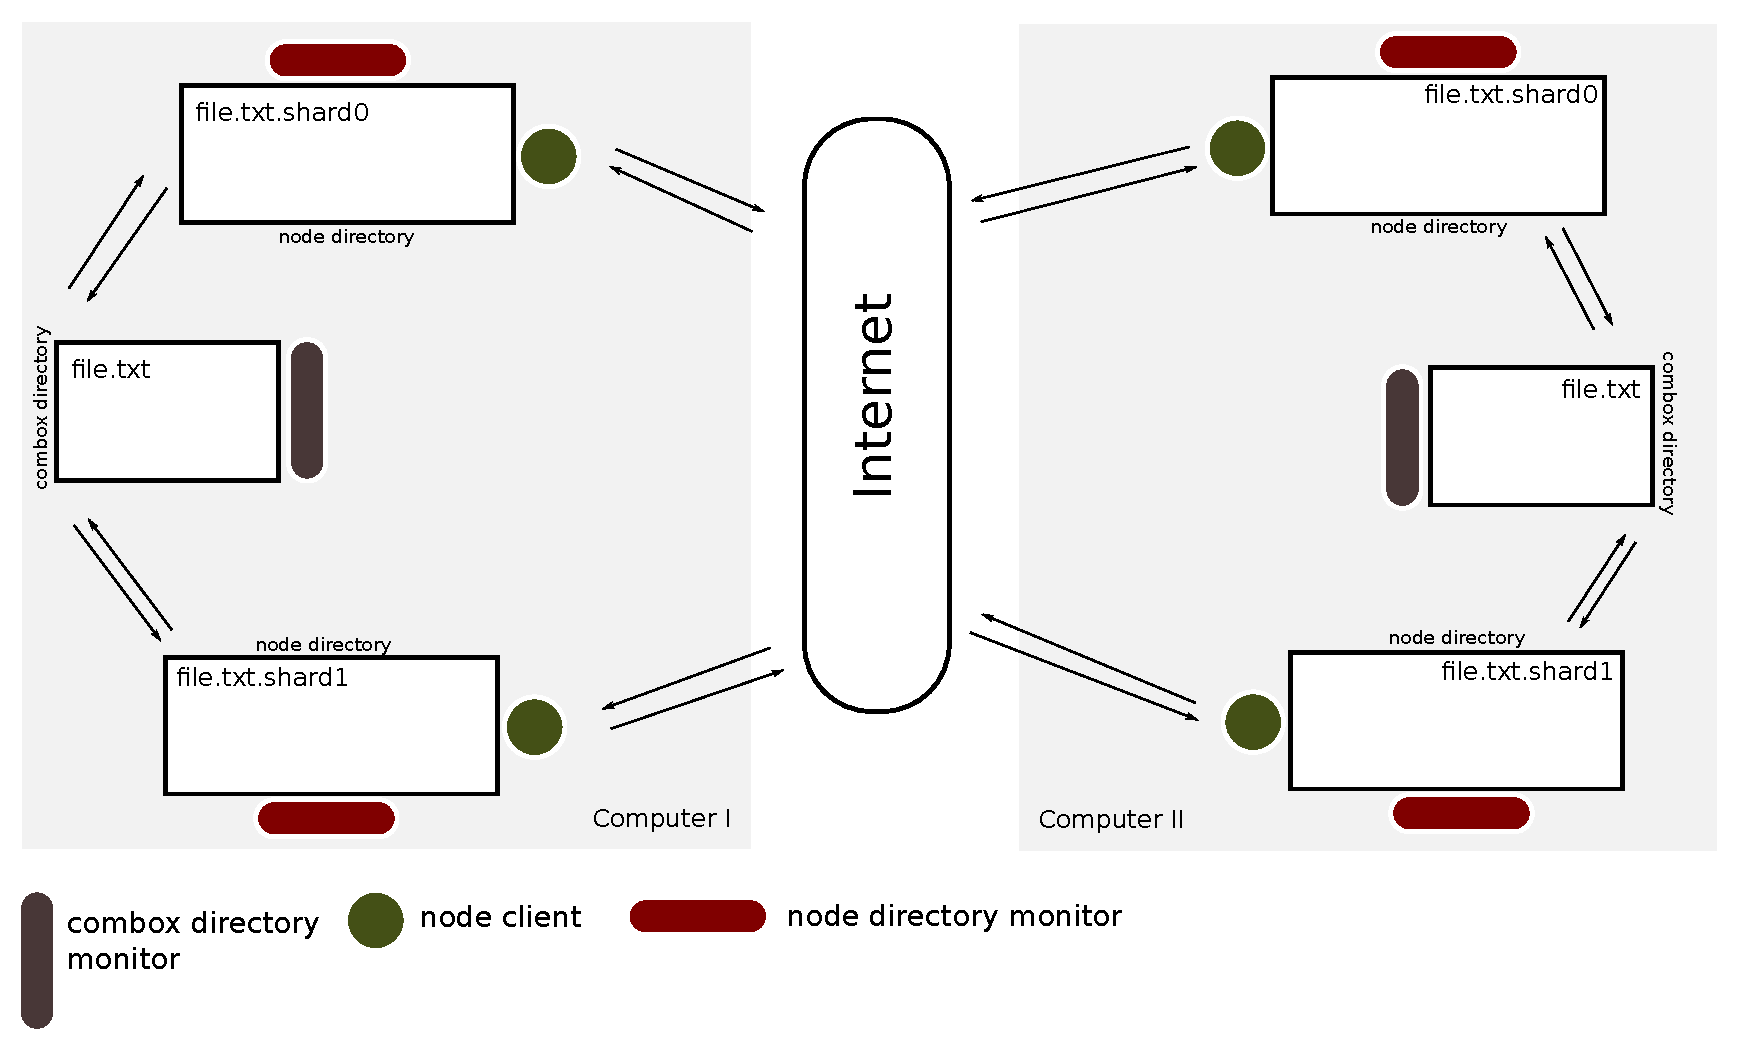
\includegraphics[scale=0.6]{3-combox-structure}
  \caption{High level overview of how file creation works when combox
    is setup on two computers.}
  \label{fig:3-combox-structure}
\end{figure}

Now, when the user moves to their second computer, the node clients
(Dropbox client and the Google Drive client) will sync the new
encrypted shards to their respective directories. Once the encrypted
shards are synced to the node directories, combox will pick the
encrypted shards -- \verb+humans.txt.shard0+, \verb+humans.txt.shard1+
-- decrypt them and reconstruct into \verb+humans.txt+ and place it in
the respective location under the combox directory;
Fig. \ref{fig:3-combox-structure} illustrates this. The process is
similar for file modification, deletion and rename/move.

\subsection{combox configuration}\label{sec:3-combox-config}

The combox configuration wizard triggers automatically when combox
finds that it is not configured. The combox configuration wizard
configures the combox directory; asks the user to point to the
location of the node directories; and reads the key (passphrase) to be
used to encrypt file shards that are spread across the node
directories. The combox configuration is written to
\verb+$HOME/.combox/config.yaml+. This YAML configuration file can be
manually edited by the user.

The \verb+config_cb+
\footnote{https://git.ricketyspace.net/combox/tree/combox/config.py?id=fb7fdd21\#n90}
function in the \verb+combox.config+ module is responsible for
carrying out the combox configuration. Prior to version \verb+0.2.0+,
the combox configuration was purely done through the Command Line
Interface (CLI). From \verb+0.2.0+ on wards, by default, the combox
configuration is done through a graphical interface; it is still
possible to configure combox through the CLI with the \verb+--cli+
switch.

A demo of combox configuration using the graphical interface on
GNU/Linux can be viewed
\url{https://ricketyspace.net/combox/combox-config-gui-glued-gnu.webm}.
T he same demo of combox configuration using the graphical interface
on OS X can be viewed
\url{https://ricketyspace.net/combox/combox-config-gui-glued-osx.webm}.

\subsection{combox directory monitor}\label{sec:3-combox-cdirm}

combox directory monitor is an instance of
\verb+combox.events.ComboxDirMonitor+
\footnote{https://git.ricketyspace.net/combox/tree/combox/events.py?id=fb7fdd21\#n42}
monitoring the combox directory for changes. When changes are made to
the combox directory, the combox directory monitor is responsible for
correctly detecting the type of change and doing the right thing at
that instance of time.

When a file is created in the combox directory, the combox directory
monitor will take that file, split it into \verb+N+ (equal to the
number of node directories) shards, encrypt the shards, spread the
encrypted shards to the node directories, and finally store the hash
of the file in the local combox data store.

When a file is modified in the combox directory, the combox directory
monitor will take that modified file, split it into \verb+N+ (equal to
the number of node directories) shards, encrypt the shards, spread the
encrypted shards to the node directories, and finally update the hash
of the file in the local combox data store.

When a file is deleted in the combox directory, the combox directory
monitor will remove the encrypted shards of the file in the node
directories and get rid of the file's hash from the local combox data
store.

When a file is moved/renamed in the combox directory, the combox
directory monitor will move/rename encrypted shards in all the node
directories, remove the file's hash from the local combox data store
and store the hash of file under its new name.

\subsection{Node directory monitor}\label{sec:3-combox-nodirm}

Node directory monitor is an instance of
\verb+combox.events.NodeDirMonitor+
\footnote{https://git.ricketyspace.net/combox/tree/combox/events.py?id=fb7fdd21\#n352}
that monitors a node directory. When changes are made to the node
directory, the node directory monitor is responsible for correctly
detecting the type of change and doing the right thing at that
instance of time. Each node directory has a dedicated node directory
monitor. If there are 2 node directories, then combox will instantiate
2 node directory monitors.

When an encrypted shard is created in the node directory due to a file
created on another computer, the node directory first checks if the
respective file' encrypted shard(s) has/have arrived in other node
directory/directories. If all encrypted shards have arrived, then the
node directory takes all the encrypted shards, decrypts them,
reconstructs the file and puts the file in the combox directory on
this computer and stores the hash of the newly created file in the
local combox data store. If all the encrypted shards have not arrived,
then the node directory does not do anything. It must be observed here
that the node directory monitor of the last node directory which gets
the encrypted shard will be the one to perform the file reconstruction
and creation.

When an encrypted shard is modified in the node directory due to a
file modified on another computer, the node directory first checks if
the respective file' modified encrypted shard(s) has/have arrived in
other node directory/directories. If all modified encrypted shards
have arrived, then the node directory takes all the modified encrypted
shards, decrypts them, reconstructs the file and puts the modified
version of the file in the combox directory on this computer and
updates the file's hash in the local combox data store. If all the
modified encrypted shards have not arrived, then the node directory
does not do anything. It must be observed here that the node directory
monitor of the last node directory which gets the modified encrypted
shard will be the one to perform the file reconstruction and will
place the modified file in the combox directory.

When an encrypted shard is deleted in the node directory due to a file
deleted on another computer, the node directory first checks if the
respective file' encrypted shard(s) has/have been deleted in other
node directory/directories. If all encrypted shards have been deleted
from the node directories, then the node directory deletes the file in
the combox directory on this computer and removes its information from
the local combox data store. If all encrypted shards have not been
deleted, then the node directory does not do anything. It must be
observed here that the node directory monitor of the last node
directory in which the encrypted shard is deleted will be the one to
delete the file from the combox directory.

When an encrypted shard is moved/renamed in the node directory due to
a file moved/renamed on another computer, the node directory first
checks if the respective file' moved/renamed encrypted shard(s)
has/have arrived in other node directory/directories. If all
moved/renamed encrypted shards have arrived, then the node directory
takes all the moved/renamed encrypted shards, decrypts them,
reconstructs the moved/renamed file and puts the moved/renamed file in
the combox directory on this computer and stores the hash under the
file' new name in the local combox data store. If the all the
moved/renamed encrypted shards have not arrived, then the node
directory does not do anything. It must be observed here that the node
directory monitor of the last node directory which gets the
moved/renamed encrypted shard will be the one to perform the file
reconstruction and will place the moved/renamed file in the combox
directory.

\subsection{combox data store}\label{sec:3-combox-db}

To ``keep it simple, stupid'', combox tracks bare minimum information
about the files that are stored in the combox directory, depending on
file system events to do the right thing when changes takes place in
the combox directory.

The only information that is stored in the combox data store with
regards to a file in the combox directory is its SHA-512 hash. The
SHA-512 hash of a file is enough information to detect changes in the
file. In the data store, there are also four dictionaries --
\verb+file_moved+, \verb+file_deleted+, \verb+file_created+,
\verb+file_modified+ -- which track the number of shards of a file
that were moved/deleted/created/modified due the respective file being
moved/deleted/created/modified on another computer. These four
dictionaries are primarily used by the \verb+NodeDirMonitor+ to detect
remote file movement/deletion/creation/modification and triggering
file reconstruction from the encrypted shards at the right time.

The data store is a JSON file on the disk, stored by default at \\
\verb+$HOME/.combox/silo.db+. The \verb+combox.silo.ComboxSilo+
\footnote{https://git.ricketyspace.net/combox/tree/combox/silo.py?id=v0.2.2\#n29}
is the sole interface to read from and write to the data store. The
data store is primarily accessed and modified by the combox directory
monitor (\verb+ComboxDirMonitor+) and the node directory monitor
(\verb+NodeDirMonitor+) through a shared \verb+threading. Lock+ that
ensures that only one entity \footnote{An entity can be the combox
  directory monitor or one of the node directory monitors} can
access/modify the database at a time.

Below is an illustration of the structure of the combox data store:

\begin{verbatim}
{
  "/home/rsd/combox/ipsum.txt": "e3206df2bb2b3091103ab9d...",
  "/home/rsd/combox/tk-shot-osx.png": "7fcf1b44c15dd95e0...",
  "/home/rsd/combox/thgttg-21st.png": "0040eedfc3eeab546...",
  "/home/rsd/combox/lorem.txt": "5851dd7a4870ff165facb71...",
  "/home/rsd/combox/the-red-star.jpg": "4b818126d882e552...",
  "file_moved": {},
  "file_deleted": {},
  "file_created": {},
  "file_modified": {},
}
\end{verbatim}

The \verb+combox.silo.ComboxSilo+, which is the sole interface to read
from and write to the database, uses the pickleDB library
\cite{pylib:pickledb}. The pickleDB is a very basic key-value store
which allows one to store information in the JSON format.

It must be noted that the combox data store on each computer is
independent and does not communicate or make transactions with the
combox data store located in other computers.

\section{combox modules overview}

combox is spread into modules that have functions and/or
classes. Currently, combox is considerably a small program consisting
of the following files:

\begin{verbatim}
$ wc -l combox/*.py
  144 combox/cbox.py
  178 combox/config.py
  241 combox/crypto.py
  891 combox/events.py
  541 combox/file.py
  454 combox/gui.py
    0 combox/__init__.py
   71 combox/log.py
  278 combox/silo.py
   29 combox/_version.py
 2827 total
\end{verbatim}

This section gives an overview of each of the combox modules with
extreme brevity.

\begin{description}
\item[combox.cbox]
  \footnote{https://git.ricketyspace.net/combox/tree/combox/cbox.py?id=fb7fdd21}
  This module contains \verb+run_cb+ function that starts/initiates
  combox; this function creates an instance \verb+threading.Lock+ for
  combox data store access and another instance of
  \verb+threading.Lock+ which is shared by instances of
  \verb+combox.events.ComboxDirMonitor+ and
  \verb+combox.events.NodeDirMonitor+; it initializes an instance
  \verb+combox.events.ComboxDirMonitor+ that monitors the combox
  directory and an instance of \verb+combox.events.NodeDirMonitor+ for
  each node directory. This modules also houses the \verb+main+
  function that parses commandline arguments, starts combox
  configuration if needed or loads the combox configuration file to
  start running combox.
\item[combox.config]
  \footnote{https://git.ricketyspace.net/combox/tree/combox/config.py?id=fb7fdd21}
  Accommodates two import functions -- \verb+config_cb+ and
  \verb+get_nodedirs+. The \verb+config_cb+ is the combox
  configuration function that allows the user to configure combox;
  this function was designed in a such way that it could be used by
  both the commandline and graphical interfaces for configuring
  combox. The \verb+get_nodedirs+ function returns, as a list, the
  paths of the node directories; this function use used in numerous
  places in other combox modules.
\item[combox.crypto]
  \footnote{https://git.ricketyspace.net/combox/tree/combox/crypto.py?id=fb7fdd21}
  This has functions for encrypting and decrypting data; encrypting
  and decrypting shards (\verb+encrypt_shards+ and
  \verb+decrypt_shards+); a function for splitting a file into shards,
  encrypting those shards and spreading them across node directories
  (\verb+split_and_encrypt+); a function for decrypting the shards
  from the node directories, reconstructing the file from the
  decrypted shards and putting the file to the combox directory
  (\verb+decrypt_and_glue+). Functions \verb+split_and_encrypt+ and
  \verb+decrypt_and_glue+ are the two functions that that are
  extensively used by the \verb+combox.events+ module; all other
  functions in this module are pretty much helper functions for
  \verb+split_and_encrypt+ and \verb+decrypt_and_glue+ functions and
  are not used by other modules.
\item[combox.events]
  \footnote{https://git.ricketyspace.net/combox/tree/combox/events.py?id=fb7fdd21}
  This module took the most time to write and test and it is the most
  complex module in combox at the time of writing this report. It
  contains just two classes -- \verb+ComboxDirMonitor+ and
  \verb+NodeDirMonitor+. The \verb+ComboxDirMonitor+ inherits the
  \verb+watchdog.events.LoggingEventHandler+ and is responsible for
  monitoring for changes in the combox directory and doing the right
  thing when a change happens in the combox directory. The
  \verb+NodeDirMonitor+ also inherits
  \verb+watchdog.events.LoggingEventHandler+ and similarly responsible
  for monitoring a node directory and doing the right thing when a
  change happens in the node directory; subjectively,
  \verb+NodeDirMonitor+ is slightly more complex than the
  \verb+ComboxDirMonitor+.
\item[combox.file]
  \footnote{https://git.ricketyspace.net/combox/tree/combox/file.py?id=fb7fdd21}
  This is the second largest module in combox. It contains utility
  functions for reading, writing, moving files/directories, hashing
  files, splitting a file into shards, gluing shards into a file,
  manipulating directories inside combox and node directories.
\item[combox.gui]
  \footnote{https://git.ricketyspace.net/combox/tree/combox/gui.py?id=fb7fdd21}
  Contains the \verb+ComboxConfigDialog+ class; it is the graphical
  interface for configuring combox. The class uses the Tkinter library
  \cite{pylib:tkinter} for spawning graphical elements. Other
  graphical libraries including PyQt \cite{pylib:qt} were considered,
  Tkinter was chosen over others due to compatibility with all Unix,
  Unix-like systems and Microsoft Windows and it is part of the
  standard python library from python version 3 on wards.
\item[combox.log]
  \footnote{https://git.ricketyspace.net/combox/tree/combox/log.py?id=fb7fdd21}
  All the messages to \verb+stdout+ and \verb+stderr+ are sent through
  the \verb+log_i+ and \verb+log_e+ functions defined in this module.
\item[combox.silo]
  \footnote{https://git.ricketyspace.net/combox/tree/combox/silo.py?id=fb7fdd21}
  Contains the \verb+ComboxSilo+ class which is the canonical
  interface for combox for managing information about the files in the
  combox directory. Internally, the \verb+ComboxSilo+ class uses the
  pickleDB library \cite{pylib:pickledb}.
\item[combox.\_version]
  \footnote{https://git.ricketyspace.net/combox/tree/combox/\_version.py?id=fb7fdd21}
  This is \emph{private} module that contains variables that contain
  the value of the present version and release of combox. The
  \verb+get_version+ function in this module returns the full version
  number; this function used by \verb+setup.py+.
\end{description}

\section{DRY}

The core functionality of combox is to split, encrypt file shards,
spread them across node directories (Google Drive and Dropbox) and
decrypt, glue shards and put them back to the combox directory when a
file is created/modified/deleted/moved in another computer. The plan
was to use external libraries to accomplish things that fell outside
the realm of the ``core functionality of combox''. The main reason
behind this decision was to not indulge in trying to solve problems
that others have already solved.

Accordingly, the \verb+watchdog+ \cite{pylib:watchdog} library was
chosen for file monitoring. This library is compatible with Unix,
Unix-like systems and Microsoft Windows. The \verb+pycrypto+ library
\cite{pylib:pycrypto} was used for encrypting data. Combox uses AES
encryption scheme to encrypt file shards. The \verb+pickleDB+
\cite{pylib:pickledb} library was used to store information about
files in the combox directory.

Looking back, the decision to use external libraries reduced the
complexity of combox, reduced the time to complete the initial working
version of combox, and made it possible to spend more than 3 months
just testing and fixing issues in combox.

\section{Operating system compatibility}\label{3-os-compat}

combox was developed on a GNU/Linux machine. A conscious effort was
made to write the software in an operating system independent way. The
top criteria for choosing a library to use in combox was that it had
to be compatible on \emph{all} of the three major computing platforms
\footnote{GNU/Linux, OS X and, Microsoft Windows}.

Prior to the \verb+0.1.0+ release, combox was tested on OS X (See
chapter \ref{ch:4}) and OS X specific issues that were found were
eventually fixed. The initial \verb+0.1.0+ release of combox was
compatible with GNU/Linux and OS X.

After the initial release of combox, it was seen if combox would be
compatible with Microsoft Windows out of the box. it was found that:

\begin{itemize}
\item Setting up the paraphernalia to run combox was non-trivial
  \cite{doc:combox-setup-windoze}.
\item The unit tests for the \verb+combox.file+ module failed on the
  Windows Operating System.
\end{itemize}

At the time of writing the report, combox is at version \verb+0.2.3+
and it is not compatible with Microsoft Windows. Comprehensive
documentation for setting up the development environment for combox on
Microsoft Windows was written \cite{doc:combox-setup-windoze} to make
it less cumbersome for anyone who would want to work on making combox
compatible with Microsoft Windows.

\section{combox as a python package}\label{3-pypi}

Before version \verb+0.2.0+, the canonical way to install combox was
to pull the source from the \verb+git+ repository with:

\begin{verbatim}
  git clone git://ricketyspace.net/combox.git
\end{verbatim}

Then, do:

\begin{verbatim}
  cd combox
\end{verbatim}

Finally install combox with:

\begin{verbatim}
  python setup.py install
\end{verbatim}

Python has a package registry called CheeseShop \footnote{code name
  for Python Package Index, see
  https://wiki.python.org/moin/CheeseShop}.  All packages registered
at the CheeseShop can be installed using \verb+pip+ -- Python's
platform independent package management system \cite{py:pip} -- with:

\begin{verbatim}
  pip install packagename
\end{verbatim}

To make it easier for (python) users to install combox on their
machine, an effort was made to make it a python package
\cite{py:package-guide}. From version \verb+0.2.0+, combox has been
registered as a python package at the CheeseShop. (Python) Users can
now easily get a copy of combox on their machine with:

\begin{verbatim}
  pip install combox
\end{verbatim}

All versions of combox that are available through the CheeseShop are
digitally signed using the following GPG key:

\begin{verbatim}
pub   4096R/00B252AF 2014-09-08 [expires: 2017-09-07]
      Key fingerprint = C174 1162 CEED 5FE8 9954  A4B9 9DF9 7838 00B2 52AF
uid                  Siddharth Ravikumar (sravik) <sravik@bgsu.edu>
sub   4096R/09CECEDB 2014-09-08 [expires: 2017-09-07]
\end{verbatim}

All versions of combox's source are also available as a compressed
\verb+TAR+ ball and as a \verb+ZIP+ archive; they can be downloaded
from \url{https://ricketyspace.net/combox/releases.html}.


%% 4
\chapter{Testing}\label{ch:4}

\epigraph{Testing shows the presence, not the absence of
  bugs.}{\textit{Dijkstra}\cite{dijkstra69}}

\section{Unit testing}\label{sec:4-unit-testing}

The \verb+nose+\cite{pylib:nose} testing framework was used to
write unit tests for the functions and classes part of the
\verb+combox.config+, \verb+combox.crypto+, \verb+combox.events+,
\verb+combox.file+, \verb+combox.silo+ \verb+combox._version+
modules. Unit tests were not written for \verb+combox.cbox+,
\verb+combox.gui+, \verb+combox.combox.log+ modules.

Unit tests for combox become reality by pure serendipity. During the
time, when I started working on combox, I was learning to use the
\verb+nose+ library to unit test python code. Since, \verb+combox+ was
being written in python, I started making it a norm to write unit
tests for functions and classes in combox modules.

As mentioned before, unit tests were not written for some modules
either because it would make no sense to write one (for the
\verb+combox.cbox+ module, for instance, which basically uses
functions and classes defined in other modules to run combox) or it
was not clear how to write unit tests it (the \verb+combox.gui+
contains just the \verb+ComboxConfigDialog+ a graphical front-end
which uses the configuration function defined in the
\verb+combox.config+ module to complete the combox configuration based
on the user input).

It must be noted here that pure Test Driven Development (TDD) was not
observed -- most of the time the function/class was written before the
its corresponding test was written.

\subsection{Benefits}

While writing unit tests definitely increased the time to write a
particular feature, it enabled me to immediately check if a feature
worked as it should for the given use case or given set of inputs.

With the benefit of hindsight, unit tests greatly helped in testing
the compatibility of combox on OSX. Before the \verb+v0.1.0+ release,
combox's node directory monitor always assumed that a file's first
shard (\verb+shard0+) is always available; while this assumption did
not create any problems on GNU/Linux, on OS X, this assumption made
the node directory monitor to behave erratically -- this issue (bug
\#4 was immediately found when the unit tests were run for the first
time on OS X. Another instance where unit tests helped was just before
the \verb+v0.2.0+ release; major changes, including the introduction
of file locks in the \verb+ComboxDirMonitor+, were made to the
\verb+combox.events+. When the unit tests were run OS X, two tests
failed, revealing a difference in behavior of
watchdog\cite{pylib:watchdog} on GNU/Linux and OS X on file
creation\footnote{https://git.ricketyspace.net/combox/commit/?id=8c86e7c28738c66c0e04ae7886b44dbcdfc6369exo}; without unit tests, there is a high
probability that this bug would never have been found by now.

\subsection{Caveats}

Unit tests are helpful in testing the correctness of a feature for
\verb+N+ number of use cases but it does not necessarily mean the
written feature correctly behaves for use cases that the author of the
feature did not consider or did not think about while writing the
respective feature. As Dijkstra correctly observed:

Unit tests failed to reveal bugs \#4, \#5 \#6 \#7 \#5 \#10
\#11\footnote{https://git.ricketyspace.net/combox/plain/TODO.org}; these bugs were found when manually
testing combox.

\section{Manual testing}\label{sec:4-manual-testing}

The unit tests for the \verb+combox.events+ module test the
correctness of the \verb+ComboxDirMonitor+ and \verb+NodeDirMonitor+
independently; in order to comprehensively test the correctness of
both \verb+ComboxDirMonitor+ and \verb+NodeDirMonitor+, it was
required to manually test combox running on more than one computer. As
you'll see in the following subsections, several bugs were found and
fixed while doing manual testing.

Three different types of setups were used to test combox. The first
kind of setup has two GNU/Linux machines each using combox to sync
files between each other with Dropbox and Google Drive being the
nodes; the second kind of setup has a GNU/Linux machine and a OS X
machine each using combox to sync files between each other with
Dropbox and Google Drive being the nodes; the third kind of setup has
a GNU/Linux machine and OS X machine each using combox to sync files
between each other with Dropbox, Google Drive and a USB stick as
nodes.

\subsection{General setup and notes}

\begin{itemize}
\item On the GNU/Linux machines, the official Dropbox client was used
  to sync the Dropbox node directory to Dropbox'
  servers. \verb+rclone+\cite{program:rclone} was used to sync the
  Google Drive node directory to Google Drive' servers;At the time of
  testing, Google Drive did not have client for GNU/Linux.
\item On OS X, the official Dropbox client was used to sync the
  Dropbox node directory to Dropbox's servers; the official Google
  Drive client was used to sync the Google Drive node directory to
  Google Driver' servers.
\item Since combox is extremely event-driven, combox must be started
  before the Dropbox and Google Drive clients start syncing their
  respective directories (nodes).
\end{itemize}

\subsection{Testing on two GNU/Linux machines}

combox was run to two GNU/Linux machines and a file was alternatively
created/modified/renamed/deleted on an of the GNU/Linux machine and it
was verified if the respective file was also
created/modified/renamed/deleted on the other GNU/Linux machine. One
of the GNU/Linux machine (\verb+lyra)+ was a virtual machine running
Debian GNU/Linux stable (version 8.x); the other GNU/Linux machine
(\verb+grus+) was a physical machine running Debian GNU/Linux
testing. The node directories to scatter the files' shards were the
Dropbox directory and Google Drive directory. The official Dropbox
client was used to automatically sync files from the Dropbox directory
to the Dropbox' server; \verb+rclone+\cite{program:rclone} was used to
sync files from Google Drive directory to Google Drive' server.

\subsubsection{Issues found}\label{ch-4-2gnus-issues}

\begin{itemize}
\item Some editors, especially on POSIX complaint systems, create
  backup version of the file being edited. combox was detecting this
  backup file as a ``new file'' and it split it into shards, encrypted
  the shards and scattered the shards across the node directories. The
  right thing for combox to do was to ignore these backup files and do
  nothing about them. This issue was fixed on
  \verb+2015-09-29+\footnote{https://git.ricketyspace.net/combox/plain/TODO.org}. Now
  the \verb+ComboxDirMonitor+, on a ``file created'' or ``file
  modified'' event, returns from the \verb+on_created+ or
  \verb+on_modified+ callback when it finds that the file is a
  backup/temporary file.
\item Dropbox client maintains the \verb+.dropbox.cache+ directory
  under the root of the Dropbox directory.

  \begin{itemize}
  \item When a file (shard) was created on another computer, the
    Dropbox client pulls the new file (shard) to this computer into
    \verb+.dropbox.cache+ as a temporary file and then moves the new
    file (shard) to its respective location with the appropriate name.
  \item When a file (shard) was modified on another computer, the
    Dropbox client pulls the modified file (shard) to this computer
    into the \verb+.dropbox.cache+ as a temporary file; moves the old
    version of the file (shard) under the Dropbox directory into the
    \verb+.dropbox.cache+; finally moves the updated copy of the file,
    stored as a temporary file, into the Dropbox directory to its
    respective location with the appropriate name.
  \item When a file (shard) was deleted on another computer, the
    Dropbox client moves the delete file into the
    \verb+.dropbox.cache+ directory on this computer.
  \end{itemize}

  All of the above behavior of the Dropbox client epically broke
  combox. Commits \verb+3d714c5+ to
  \verb+6e1133f+\footnote{https://git.ricketyspace.net/combox/log/?qt=range\&q=3d714c5..6e1133f}
  fixed combox by making it aware of Dropbox's client behavior.
\end{itemize}

\subsubsection{Demo}

Demo of combox being used on two GNU/Linux machines can be viewed at
\url{https://ricketyspace.net/combox/combox-2-gnus.webm}.

\verb+lyra+ (virtual machine) and \verb+grus+ (bare-metal) are the two
GNU/Linux machines being used for the demo.

Description of what happens in the demo follows:

 - (lyra) install combox.

 - (lyra) run combox (test mode).

 - (lyra) create file \verb+walden.pond+ with content ``It must be
 beautiful there''.

 - (lyra) sync Google Drive using \verb+rclone+.

 - (grus) sync Google Drive using \verb+rclone+.

 - (grus) git pull latest copy of combox.

 - (grus) install combox 

 - (grus) run combox (testing mode).

 - (grus) verify that \verb+walden.pond+ was create on this machine.

 - (grus) append 'Peaceful too.' to \verb+walden.pond+.

 - (grus) sync Google Drive using \verb+rclone+.

 - (lyra) sync Google Drive using \verb+rclone+.

 - (lyra) verify that the latest copy of \verb+walden.pond+ is there
 in the combox directory; it should contain 'Peaceful too.' in the
 last line.

 - (lyra) append ``I've a dream'' to \verb+walden.pond+.

 - (lyra) sync Google Drive using \verb+rclone+.

 - (grus) sync Google Drive using \verb+rclone+.

 - (grus) verify that the latest copy of \verb+walden.pond+ is there
 in the combox directory; it should contain ``I've a dream'' in the
 last line.

 - (grus) remove \verb+walden.pond+ from combox directory.

 - (grus) sync Google Drive using \verb+rclone+.

 - (lyra) sync Google Drive using \verb+rclone+.

 - (lyra) verify that \verb+walden.pond+ is removed from the combox
 directory.

 - (grus) open dropbox and Google drive accounts from the web browser.

 - (lyra) create file \verb+manufacturing.consent.+ with content ``Chomsky stuff?''.

 - (lyra) sync Google Drive using \verb+rclone+.

 - (grus) sync Google Drive using \verb+rclone+.

 - (grus) verify that \verb+manufacturing.consent+ was created in the
 combox directory.

 - (grus) verify that the shards of \verb+manufacturing.consent+ were
 created on Dropbox and Google Drive through the web browser.

\subsection{Testing on a GNU/Linux and an OS X machine}

combox was run on a GNU/Linux machine and an OS X machine and a file
was alternatively created/modified/renamed/deleted on one of the
machine and it was verified if the respective file was also
created/modified/renamed/deleted on the other machine. The GNU/Linux
machine was a virtual machine (\verb+lyra+) running Debian GNU/Linux
stable; the OS X machine was on Mavericks (10.9) during the initial
stage of testing, later it was upgraded to Yosemite (10.10). The node
directories to scatter files' shards were the Dropbox directory and
the Google Drive directory. The official Dropbox client was used to
automatically sync files from the Dropbox directory to the Dropbox'
server on both the GNU/Linux machine and the OS X machine; the
official Google Drive client was used to automatically sync files from
the Google Drive directory to Google Drive' server on OS X and
\verb+rclone+\cite{program:rclone} was used to sync files from the
Google Drive directory to Google Drive's server on GNU/Linux.

\subsubsection{Issues found}

\begin{itemize}
\item When a file was modified on another computer, on this computer
  combox assumed that first shard (shard0) will be updated first and
  also counted on the existence of the first shard (shard0). It was
  observed that the order in which the shards were updated were
  unpredictable on this computer and if the first shard (shard0) was
  stored in the Dropbox directory, it will momentarily disappear
  before the most updated shard becomes available in the Dropbox
  directory; this broke combox. This issue was fixed on
  2015-08-25\footnote{https://git.ricketyspace.net/combox/commit/?id=d5b52030348d40600b4c9256f76e5183a85fbb17}. This issue is not got to do with
  the nature of the setup but it is related to the Dropbox's behavior
  elaborated in section \ref{ch-4-2gnus-issues}.
\item The official Google Drive client when it pulls an updated
  version of the file from Google Drive' server, instead directly
  updating the respective file on the computer, it deletes the older
  version of the file and creates the latest version of the file at
  the respective location in the Google Drive directory; this behavior
  of the Google Drive confused and broke combox. This issue was fixed
  2015-09-06 by making combox under the official Google Client's
  behavior\footnote{https://git.ricketyspace.net/combox/commit/?id=37385a90f90cb9d4dfd13d9d2e3cbcace8011e9e}.
\item When a non-empty directory was move/renamed on another computer,
  the old directory was not getting properly deleted on this computer;
  this was happening because the files under the directory being
  renamed were not deleted when it was time for \verb+NodeDirMonitor+
  to \verb+rmdir+ the old directory. This issue again is not specific
  to the nature of the setup but was found while testing combox on
  this setup. This issue was fixed on
  2015-09-12\footnote{https://git.ricketyspace.net/combox/commit/?id=9d14db03da5d10d5ab0d7cc76b20e7b1ed5523bf}.
\item It was found that \verb+combox.file.rm_path+ function failed
  when it was given a non-existent path to remove; this issue was
  fixed on 2015-09-12\footnote{https://git.ricketyspace.net/combox/commit/?id=422238eb4904de14842221fa09a2b4028801afb1}.
\end{itemize}

\subsubsection{Demo}

Demo of combox being used on a GNU/Linux machine and OS X machine can
be viewed at \url{https://ricketyspace.net/combox/combox-gnu-osx.webm}

\verb+lyra+ is the GNU/Linux (virtual) machine and
\verb+dhcp-129-1-66-1+ is the OS X machine that is being used for the
demo. The OS X machine is accessed through VNC\cite{article:vnc}.

Description of what happens in the demo follows:

  - (\verb+lyra+) create file \verb+cat.stevens+ with content ``peace train''.

  - (\verb+lyra+) sync Google Drive using \verb+rclone+.

  - (\verb+dhcp-129-1-66-1+) verify that file \verb+cat.stevens+ is
  created with content ``peace train''.

  - (\verb+dhcp-129-1-66-1+) append string ``moonshadow'' to file
  \verb+cat.stevens+.

  - (\verb+lyra+) sync Google Drive using \verb+rclone+.

  - (\verb+lyra+) verify that the file \verb+cat.stevens+ was updated
  (modified); last line must have the string ``moonshadow''.

  - (\verb+lyra+) append string ``father and son'' to the file
  \verb+cat.stevens+.

  - (\verb+lyra+) sync Google Drive using \verb+rclone+.

  - (\verb+dhcp-129-1-66-1+) verify that the file \verb+cat.stevens+
  was updated (modified); last line must have the string ``father and
  son''.

  - (\verb+dhcp-129-1-66-1+) rename file \verb+cat.stevens+ to
  \verb+yusuf.islam+

  - (\verb+lyra+) sync Google Drive using \verb+rclone+.

  - (\verb+lyra+) verify that the file \verb+cat.stevens+ was renamed
  to \verb+yusuf.islam+.

\subsection{Testing with a USB stick as a node}

combox was run on a GNU/Linux machine and an OS X machine and a file
was alternatively created/modified/deleted on one of the machine and
it was verified if the repsective file was also
create/modified/deleted on the other machine. The GNU/Linux machine
was a physical machine (\verb+grus+) running Debian GNU/Linux stable;
The OS X machine was on Mavericks (10.9). The node directories to
scatter files' shards were the Dropbox directory, Google Drive
directory and the USB stick (\verb+ZAPHOD+, FAT filesystem). The
official Dropbox client was used to automatically sync files from
Dropbox directory to Dropbox' server on both the GNU/Linux machine and
OS X machine; the official Google Drive client was used to
automatically sync files from the Google Drive directory to Google
Drive' server on OS X and \verb+rclone+\cite{program:rclone} was used
to sync files from the Google Drive directory to Google Drive's server
on GNU/Linux; the same USB stick (\verb+ZAPHOD+) was used on bothe
GNU/Linux and Dropbox to store the third shard (shard2) of a file.

\subsubsection{Caveats}

\begin{itemize}
\item When a removable USB disk is used as a node, combox must be
  turned off before ejecting/unmounting the USB disk; combox does not
  expect a node directory to disappear when it is running, if the USB
  disk is removed when combox is running, then combox goes to a
  undefined state.

\item When a file modified on machine A is synced to machine B, combox
  must be turned on first before turning on Dropbox and Google Drive
  clients and the shard in the USB disk needs to be ``touched'' for
  combox to detect that the file was modified on the remote computer
  and update the file locally on this machine.

\item File rename/move does not work. To make it work, core
  functionality of combox must be re-written.
\end{itemize}

\subsubsection{Demo}

Demo of combox being used with a USB stick as the third node can be
view at \url{https://ricketyspace.net/combox/combox-usb-node-demo.webm}

\verb+grus+ is the GNU/Linux machine and \verb+dhcp-129-1-66-1+ is the
OS X machine that is being used for the demo. \verb+ZAPHOD+ is the
FAT32 USB stick used as the third node.

Description of what happens in the demo follows:

  - (\verb+grus+) start combox.

  - (\verb+grus+) create a file called \verb+simon.and.garfunkel+ with
  content ``the boxer''.

  - (\verb+grus+) sync Google Drive using \verb+rclone+.

  - (\verb+grus+) stop combox.

  - (\verb+grus+) unmount USB stick (\verb+ZAPHOD+) from \verb+grus+.

  - (\verb+dhcp-129-1-66-1+) mount USB stick (\verb+ZAPHOD+) to
  (\verb+dhcp-129-1-66-1+).

  - (\verb+dhcp-129-1-66-1+) start Dropbox client.

  - (\verb+dhcp-129-1-66-1+) start Google Drive client.

  - (\verb+dhcp-129-1-66-1+) start combox.

  - (\verb+dhcp-129-1-66-1+) verify that the file
  \verb+simon.and.garfunkel+ with content ``the boxer'' was created.

  - (\verb+dhcp-129-1-66-1+) append string ``mrs. robinson'' to file
  \verb+simon.and.garfunkel+.

  - (\verb+dhcp-129-1-66-1+) stop combox.

  - (\verb+dhcp-129-1-66-1+) stop Google Drive client.

  - (\verb+dhcp-129-1-66-1+) stop Dropbox client.

  - (\verb+dhcp-129-1-66-1+) unmount the USB stick (\verb+ZAPHOD+)
  from (\verb+dhcp-129-1-66-1+).

  - (\verb+grus+) mount the USB stick (\verb+ZAPHOD+) to
  (\verb+grus+).

  - (\verb+grus+) start combox.

  - (\verb+grus+) start Dropbox client.

  - (\verb+grus+) sync Google Drive using \verb+rclone+.

  - (\verb+grus+) touch \verb+simon.and.garfunkel.shard2+ in the USB
  stick (\verb+ZAPHOD+).

  - (\verb+grus+) verify that the file \verb+simon.and.garfunkel+ is
  updated; the last line must contain the string ``mrs. robinson''.

  - (\verb+grus+) remove the file \verb+simon.and.garfunkel+.

  - (\verb+grus+) sync Google Drive using \verb+rclone+.

  - (\verb+grus+) unmount the USB stick (\verb+ZAPHOD+) from
  (\verb+grus+).

  - (\verb+grus+) stop Dropbox client.

  - (\verb+dhcp-129-1-66-1+) mount the USB stick (\verb+ZAPHOD+) to
  (\verb+dhcp-129-1-66-1+).

  - (\verb+dhcp-129-1-66-1+) start Google Drive client.

  - (\verb+dhcp-129-1-66-1+) start Dropbox client.

  - (\verb+dhcp-129-1-66-1+) start combox.

  - (\verb+dhcp-129-1-66-1+) verify that the file
  \verb+simon.and.garfunkel+ was deleted.


\section{Stress testing}

Large number of files of different sizes were dumped to the combox
directory between an one second interval to see how combox responds to
high load. The file dump size was varied from \verb+424.798190MiB+ (27
files) to \verb+10800.000000MiB+ (180 files); the average time taken
to split a file and the total time to process all files were
calculated for each dump.

Stress testing was first done on \verb+2015-11-08+. In mid November
the \verb+ComboxDirMonitor+ was drastically modified to make it use
the file Lock shared the instances of
\verb+NodeDirMonitor+\footnote{https://git.ricketyspace.net/combox/commit/?id=5aa1ba0c1dcad62931ba27bb66bf115233086d6c}; my hunch was that this
change in \verb+ComboxDirMonitor+ directly affected the performance of
combox and therefore the results that were got from stress testing on
\verb+2015-11-08+ would no longer be valid. Stress testing was again
done on \verb+2016-01-16+; the results of this stress test are in
sections \ref{4-st-424} to \ref{4-st-10800}, section \ref{4-st-tu}
gives information about the tools used for stress testing, section
\ref{4-st-o} contains the observations and comparisons between this
stress test and the one done on \verb+2015-11-08+, lastly section
\ref{4-st-if} reveals the issues that were found with combox by virtue
of doing the stress tests.

\subsection{flac dump (27 files - 424.798190MiB)}\label{4-st-424}

\begin{center}
\begin{table}[h]
\begin{tabular}{ll}
field & value\\
\hline
delay between a file dump & 1s\\
start time of processing & 11:00:54\\
end time of processing & 11:01:38\\
total time taken to process all files & 00:00:44\\
no. of files & 27\\
total size of all files & 445433187.000000 bytes (424.798190MiB)\\
avg. file size & 16497525.000000 bytes (15.733266MiB)\\
avg. time to split and encrypt a file & 352.583370 ms\\
\end{tabular}
\caption{4424.798190MiB flac dump results}
\end{table}
\end{center}

\subsubsection{Differences from previous stress test (2015-11-08)}

\begin{itemize}
\item Total time to process all files was faster by 1min3secs.
\item Average time to split and encrypt a file reduced by
  28.337963000000002ms.
\end{itemize}

\subsection{20MiB - 90MiB dump (27 files - 1620.000000MiB)}\label{4-st-1620}

\begin{center}
\begin{table}[h]
\begin{tabular}{ll}
field & value\\
\hline
delay between a file dump & 1s\\
start time of processing & 12:26:45\\
end time of processing & 12:29:07\\
total time taken to process all files & 00:02:22\\
no. of files & 27\\
total size of all files & 1698693120.000000 bytes (1620.000000MiB)\\
avg. file size & 62914560.000000 bytes (60.000000MiB)\\
avg. time to split and encrypt a file & 2670.596556ms\\
\end{tabular}
\caption{1620.000000MiB dump results}
\end{table}
\end{center}

\subsubsection{Differences from previous stress test (2015-11-08)}

\begin{itemize}
\item Total time to process all files was slower by 4secs.
\item Average time to split and encrypt a file reduced by
   25.52536999999984ms.
\end{itemize}

\subsection{20MiB - 90MiB dump (99 files - 5940.000000MiB)}\label{4-st-5940}

\begin{center}
\begin{table}[h]
\begin{tabular}{ll}
field & value\\
\hline
delay between a file dump & 1s\\
start time of processing & 13:10:16\\
end time of processing & 13:19:26\\
total time taken to process all files & 00:09:10\\
no. of files & 99\\
total size of all files & 6228541440.000000 bytes (5940.000000MiB)\\
avg. file size & 62914560.000000 bytes (60.000000MiB)\\
avg. time to split and encrypt a file & 2979.647586ms\\
\end{tabular}
\caption{5940.000000MiB dump results}
\end{table}
\end{center}

\subsubsection{Differences from previous stress test (2015-11-08)}

\begin{itemize}
\item Total time to process all files was faster by 59secs.
\item Average time to split and encrypt a file increased by
  206.20906100000002ms.
\end{itemize}

\subsection{20MiB - 90MiB dump (180 files - 10800.000000MiB)}\label{4-st-10800}

\begin{center}
\begin{table}[h]
\begin{tabular}{ll}
field & value\\
\hline
delay between a file dump & 1s\\
start time of processing & 13:42:06\\
end time of processing & 14:00:10\\
total time taken to process all files & 00:18:04\\
no. of files & 180\\
total size of all files & 11324620800.000000 bytes (10800.000000MiB)\\
avg. file size & 62914560.000000 bytes (60.000000MiB)\\
avg. time to split and encrypt a file & 3423.087539ms\\
\end{tabular}
\caption{10800.000000MiB dump results}
\end{table}
\end{center}

\subsubsection{Differences from previous stress test (2015-11-08)}

\begin{itemize}
\item Total time to process all files was slower by 1min2secs
\item Average time to split and encrypt a file increased by
  399.87623299999996ms.
\end{itemize}

\subsection{Tools used}\label{4-st-tu}

The \verb+dump+ script\footnote{https://git.ricketyspace.net/combox-paper/plain/dumper/dump} was used to dump files to
the combox directory between one second intervals; a night of Emacs
Lisp indulgence made it possible to quickly slurp the required data
from the combox output and calculate the average time to split and
encrypt a file and the total amount of time taken to process the files
for a given dump\footnote{https://git.ricketyspace.net/combox-paper/plain/scripts/dumps.el}; lastly \verb+org-mode+ was
used to document all data gathered during stress
testing\footnote{https://git.ricketyspace.net/combox-paper/plain/notes/benchmarks.org}.

\subsection{Observations}\label{4-st-o}

\begin{figure}[h]
\centering
% GNUPLOT: LaTeX picture
\setlength{\unitlength}{0.240900pt}
\ifx\plotpoint\undefined\newsavebox{\plotpoint}\fi
\sbox{\plotpoint}{\rule[-0.200pt]{0.400pt}{0.400pt}}%
\begin{picture}(1535,944)(0,0)
\sbox{\plotpoint}{\rule[-0.200pt]{0.400pt}{0.400pt}}%
\put(171.0,131.0){\rule[-0.200pt]{313.893pt}{0.400pt}}
\put(171.0,131.0){\rule[-0.200pt]{4.818pt}{0.400pt}}
\put(151,131){\makebox(0,0)[r]{0}}
\put(1454.0,131.0){\rule[-0.200pt]{4.818pt}{0.400pt}}
\put(171.0,260.0){\rule[-0.200pt]{313.893pt}{0.400pt}}
\put(171.0,260.0){\rule[-0.200pt]{4.818pt}{0.400pt}}
\put(151,260){\makebox(0,0)[r]{200}}
\put(1454.0,260.0){\rule[-0.200pt]{4.818pt}{0.400pt}}
\put(171.0,388.0){\rule[-0.200pt]{313.893pt}{0.400pt}}
\put(171.0,388.0){\rule[-0.200pt]{4.818pt}{0.400pt}}
\put(151,388){\makebox(0,0)[r]{400}}
\put(1454.0,388.0){\rule[-0.200pt]{4.818pt}{0.400pt}}
\put(171.0,517.0){\rule[-0.200pt]{313.893pt}{0.400pt}}
\put(171.0,517.0){\rule[-0.200pt]{4.818pt}{0.400pt}}
\put(151,517){\makebox(0,0)[r]{600}}
\put(1454.0,517.0){\rule[-0.200pt]{4.818pt}{0.400pt}}
\put(171.0,646.0){\rule[-0.200pt]{313.893pt}{0.400pt}}
\put(171.0,646.0){\rule[-0.200pt]{4.818pt}{0.400pt}}
\put(151,646){\makebox(0,0)[r]{800}}
\put(1454.0,646.0){\rule[-0.200pt]{4.818pt}{0.400pt}}
\put(171.0,774.0){\rule[-0.200pt]{313.893pt}{0.400pt}}
\put(171.0,774.0){\rule[-0.200pt]{4.818pt}{0.400pt}}
\put(151,774){\makebox(0,0)[r]{1000}}
\put(1454.0,774.0){\rule[-0.200pt]{4.818pt}{0.400pt}}
\put(171.0,903.0){\rule[-0.200pt]{313.893pt}{0.400pt}}
\put(171.0,903.0){\rule[-0.200pt]{4.818pt}{0.400pt}}
\put(151,903){\makebox(0,0)[r]{1200}}
\put(1454.0,903.0){\rule[-0.200pt]{4.818pt}{0.400pt}}
\put(171.0,131.0){\rule[-0.200pt]{0.400pt}{185.975pt}}
\put(171.0,131.0){\rule[-0.200pt]{0.400pt}{4.818pt}}
\put(171,90){\makebox(0,0){0}}
\put(171.0,883.0){\rule[-0.200pt]{0.400pt}{4.818pt}}
\put(388.0,131.0){\rule[-0.200pt]{0.400pt}{171.280pt}}
\put(388.0,883.0){\rule[-0.200pt]{0.400pt}{4.818pt}}
\put(388.0,131.0){\rule[-0.200pt]{0.400pt}{4.818pt}}
\put(388,90){\makebox(0,0){2000}}
\put(388.0,883.0){\rule[-0.200pt]{0.400pt}{4.818pt}}
\put(605.0,131.0){\rule[-0.200pt]{0.400pt}{171.280pt}}
\put(605.0,883.0){\rule[-0.200pt]{0.400pt}{4.818pt}}
\put(605.0,131.0){\rule[-0.200pt]{0.400pt}{4.818pt}}
\put(605,90){\makebox(0,0){4000}}
\put(605.0,883.0){\rule[-0.200pt]{0.400pt}{4.818pt}}
\put(823.0,131.0){\rule[-0.200pt]{0.400pt}{171.280pt}}
\put(823.0,883.0){\rule[-0.200pt]{0.400pt}{4.818pt}}
\put(823.0,131.0){\rule[-0.200pt]{0.400pt}{4.818pt}}
\put(823,90){\makebox(0,0){6000}}
\put(823.0,883.0){\rule[-0.200pt]{0.400pt}{4.818pt}}
\put(1040.0,131.0){\rule[-0.200pt]{0.400pt}{185.975pt}}
\put(1040.0,131.0){\rule[-0.200pt]{0.400pt}{4.818pt}}
\put(1040,90){\makebox(0,0){8000}}
\put(1040.0,883.0){\rule[-0.200pt]{0.400pt}{4.818pt}}
\put(1257.0,131.0){\rule[-0.200pt]{0.400pt}{185.975pt}}
\put(1257.0,131.0){\rule[-0.200pt]{0.400pt}{4.818pt}}
\put(1257,90){\makebox(0,0){10000}}
\put(1257.0,883.0){\rule[-0.200pt]{0.400pt}{4.818pt}}
\put(1474.0,131.0){\rule[-0.200pt]{0.400pt}{185.975pt}}
\put(1474.0,131.0){\rule[-0.200pt]{0.400pt}{4.818pt}}
\put(1474,90){\makebox(0,0){12000}}
\put(1474.0,883.0){\rule[-0.200pt]{0.400pt}{4.818pt}}
\put(171.0,131.0){\rule[-0.200pt]{0.400pt}{185.975pt}}
\put(171.0,131.0){\rule[-0.200pt]{313.893pt}{0.400pt}}
\put(1474.0,131.0){\rule[-0.200pt]{0.400pt}{185.975pt}}
\put(171.0,903.0){\rule[-0.200pt]{313.893pt}{0.400pt}}
\put(30,599){\makebox(0,0){time taken (s)}}
\put(822,29){\makebox(0,0){data processed (MiB)}}
\put(691,862){\makebox(0,0)[r]{time to process all files}}
\put(711.0,862.0){\rule[-0.200pt]{24.090pt}{0.400pt}}
\put(217,159){\usebox{\plotpoint}}
\multiput(217.00,159.58)(1.034,0.499){123}{\rule{0.925pt}{0.120pt}}
\multiput(217.00,158.17)(128.079,63.000){2}{\rule{0.463pt}{0.400pt}}
\multiput(347.00,222.58)(0.892,0.500){523}{\rule{0.813pt}{0.120pt}}
\multiput(347.00,221.17)(467.312,263.000){2}{\rule{0.407pt}{0.400pt}}
\multiput(816.00,485.58)(0.770,0.500){683}{\rule{0.716pt}{0.120pt}}
\multiput(816.00,484.17)(526.514,343.000){2}{\rule{0.358pt}{0.400pt}}
\put(217,159){\makebox(0,0){$+$}}
\put(347,222){\makebox(0,0){$+$}}
\put(816,485){\makebox(0,0){$+$}}
\put(1344,828){\makebox(0,0){$+$}}
\put(761,862){\makebox(0,0){$+$}}
\put(171.0,131.0){\rule[-0.200pt]{0.400pt}{185.975pt}}
\put(171.0,131.0){\rule[-0.200pt]{313.893pt}{0.400pt}}
\put(1474.0,131.0){\rule[-0.200pt]{0.400pt}{185.975pt}}
\put(171.0,903.0){\rule[-0.200pt]{313.893pt}{0.400pt}}
\end{picture}

\caption{time to process all files}
\label{fig:4-st-tt}
\end{figure}

\begin{figure}[h]
\centering
% GNUPLOT: LaTeX picture
\setlength{\unitlength}{0.240900pt}
\ifx\plotpoint\undefined\newsavebox{\plotpoint}\fi
\begin{picture}(1535,944)(0,0)
\sbox{\plotpoint}{\rule[-0.200pt]{0.400pt}{0.400pt}}%
\put(281.0,131.0){\rule[-0.200pt]{287.394pt}{0.400pt}}
\put(281.0,131.0){\rule[-0.200pt]{4.818pt}{0.400pt}}
\put(261,131){\makebox(0,0)[r]{0}}
\put(1454.0,131.0){\rule[-0.200pt]{4.818pt}{0.400pt}}
\put(281.0,241.0){\rule[-0.200pt]{287.394pt}{0.400pt}}
\put(281.0,241.0){\rule[-0.200pt]{4.818pt}{0.400pt}}
\put(261,241){\makebox(0,0)[r]{500}}
\put(1454.0,241.0){\rule[-0.200pt]{4.818pt}{0.400pt}}
\put(281.0,352.0){\rule[-0.200pt]{287.394pt}{0.400pt}}
\put(281.0,352.0){\rule[-0.200pt]{4.818pt}{0.400pt}}
\put(261,352){\makebox(0,0)[r]{1000}}
\put(1454.0,352.0){\rule[-0.200pt]{4.818pt}{0.400pt}}
\put(281.0,462.0){\rule[-0.200pt]{287.394pt}{0.400pt}}
\put(281.0,462.0){\rule[-0.200pt]{4.818pt}{0.400pt}}
\put(261,462){\makebox(0,0)[r]{1500}}
\put(1454.0,462.0){\rule[-0.200pt]{4.818pt}{0.400pt}}
\put(281.0,572.0){\rule[-0.200pt]{287.394pt}{0.400pt}}
\put(281.0,572.0){\rule[-0.200pt]{4.818pt}{0.400pt}}
\put(261,572){\makebox(0,0)[r]{2000}}
\put(1454.0,572.0){\rule[-0.200pt]{4.818pt}{0.400pt}}
\put(281.0,682.0){\rule[-0.200pt]{287.394pt}{0.400pt}}
\put(281.0,682.0){\rule[-0.200pt]{4.818pt}{0.400pt}}
\put(261,682){\makebox(0,0)[r]{2500}}
\put(1454.0,682.0){\rule[-0.200pt]{4.818pt}{0.400pt}}
\put(281.0,793.0){\rule[-0.200pt]{287.394pt}{0.400pt}}
\put(281.0,793.0){\rule[-0.200pt]{4.818pt}{0.400pt}}
\put(261,793){\makebox(0,0)[r]{3000}}
\put(1454.0,793.0){\rule[-0.200pt]{4.818pt}{0.400pt}}
\put(281.0,903.0){\rule[-0.200pt]{287.394pt}{0.400pt}}
\put(281.0,903.0){\rule[-0.200pt]{4.818pt}{0.400pt}}
\put(261,903){\makebox(0,0)[r]{3500}}
\put(1454.0,903.0){\rule[-0.200pt]{4.818pt}{0.400pt}}
\put(281.0,131.0){\rule[-0.200pt]{0.400pt}{185.975pt}}
\put(281.0,131.0){\rule[-0.200pt]{0.400pt}{4.818pt}}
\put(281,90){\makebox(0,0){0}}
\put(281.0,883.0){\rule[-0.200pt]{0.400pt}{4.818pt}}
\put(480.0,131.0){\rule[-0.200pt]{0.400pt}{171.280pt}}
\put(480.0,883.0){\rule[-0.200pt]{0.400pt}{4.818pt}}
\put(480.0,131.0){\rule[-0.200pt]{0.400pt}{4.818pt}}
\put(480,90){\makebox(0,0){2000}}
\put(480.0,883.0){\rule[-0.200pt]{0.400pt}{4.818pt}}
\put(679.0,131.0){\rule[-0.200pt]{0.400pt}{171.280pt}}
\put(679.0,883.0){\rule[-0.200pt]{0.400pt}{4.818pt}}
\put(679.0,131.0){\rule[-0.200pt]{0.400pt}{4.818pt}}
\put(679,90){\makebox(0,0){4000}}
\put(679.0,883.0){\rule[-0.200pt]{0.400pt}{4.818pt}}
\put(878.0,131.0){\rule[-0.200pt]{0.400pt}{171.280pt}}
\put(878.0,883.0){\rule[-0.200pt]{0.400pt}{4.818pt}}
\put(878.0,131.0){\rule[-0.200pt]{0.400pt}{4.818pt}}
\put(878,90){\makebox(0,0){6000}}
\put(878.0,883.0){\rule[-0.200pt]{0.400pt}{4.818pt}}
\put(1076.0,131.0){\rule[-0.200pt]{0.400pt}{171.280pt}}
\put(1076.0,883.0){\rule[-0.200pt]{0.400pt}{4.818pt}}
\put(1076.0,131.0){\rule[-0.200pt]{0.400pt}{4.818pt}}
\put(1076,90){\makebox(0,0){8000}}
\put(1076.0,883.0){\rule[-0.200pt]{0.400pt}{4.818pt}}
\put(1275.0,131.0){\rule[-0.200pt]{0.400pt}{185.975pt}}
\put(1275.0,131.0){\rule[-0.200pt]{0.400pt}{4.818pt}}
\put(1275,90){\makebox(0,0){10000}}
\put(1275.0,883.0){\rule[-0.200pt]{0.400pt}{4.818pt}}
\put(1474.0,131.0){\rule[-0.200pt]{0.400pt}{185.975pt}}
\put(1474.0,131.0){\rule[-0.200pt]{0.400pt}{4.818pt}}
\put(1474,90){\makebox(0,0){12000}}
\put(1474.0,883.0){\rule[-0.200pt]{0.400pt}{4.818pt}}
\put(281.0,131.0){\rule[-0.200pt]{0.400pt}{185.975pt}}
\put(281.0,131.0){\rule[-0.200pt]{287.394pt}{0.400pt}}
\put(1474.0,131.0){\rule[-0.200pt]{0.400pt}{185.975pt}}
\put(281.0,903.0){\rule[-0.200pt]{287.394pt}{0.400pt}}
\put(30,631){\makebox(0,0){avg time taken (ms)}}
\put(877,29){\makebox(0,0){total size of files processed (MiB)}}
\put(981,862){\makebox(0,0)[r]{avg. time to split \& encrypt file}}
\put(1001.0,862.0){\rule[-0.200pt]{24.090pt}{0.400pt}}
\put(323,209){\usebox{\plotpoint}}
\multiput(323.58,209.00)(0.499,2.152){235}{\rule{0.120pt}{1.818pt}}
\multiput(322.17,209.00)(119.000,507.227){2}{\rule{0.400pt}{0.909pt}}
\multiput(442.00,720.58)(3.175,0.499){133}{\rule{2.629pt}{0.120pt}}
\multiput(442.00,719.17)(424.543,68.000){2}{\rule{1.315pt}{0.400pt}}
\multiput(872.00,788.58)(2.471,0.499){193}{\rule{2.071pt}{0.120pt}}
\multiput(872.00,787.17)(478.701,98.000){2}{\rule{1.036pt}{0.400pt}}
\put(323,209){\makebox(0,0){$+$}}
\put(442,720){\makebox(0,0){$+$}}
\put(872,788){\makebox(0,0){$+$}}
\put(1355,886){\makebox(0,0){$+$}}
\put(1051,862){\makebox(0,0){$+$}}
\put(281.0,131.0){\rule[-0.200pt]{0.400pt}{185.975pt}}
\put(281.0,131.0){\rule[-0.200pt]{287.394pt}{0.400pt}}
\put(1474.0,131.0){\rule[-0.200pt]{0.400pt}{185.975pt}}
\put(281.0,903.0){\rule[-0.200pt]{287.394pt}{0.400pt}}
\end{picture}

\caption{avg. time to split and encrypt}
\label{fig:4-st-atsae}
\end{figure}


\begin{itemize}
\item Figure \ref{fig:4-st-tt} shows the time it takes combox to
  process files for a given file dump\footnote{A ``file dump'' here
    means a bunch of files copied to the combox directory between 1
    sec intervals.}. As can be observed from the graph, the total time
  taken to process all the files tends almost linearly increase with
  the increase in the size of the file dump\footnote{The ``size of the
    file dump'' is the total size of all files in a given file dump.}.
\item Figure \ref{fig:4-st-atsae} show the average time it takes
  combox to split and encrypt a file for a given file dump. There is a
  steep increase in the average time from the \verb+424.798190MiB+
  dump and the \verb+1620.000000MiB+ dump, after which the average
  time to split and encrypt a file seems to almost linearly increase;
  The main reason for this is that the average file size for dumps
  from \verb+1620.000000MiB+ to \verb+10800.000000MiB+ are the same.
\end{itemize}

\begin{figure}[h]
\centering
% GNUPLOT: LaTeX picture
\setlength{\unitlength}{0.240900pt}
\ifx\plotpoint\undefined\newsavebox{\plotpoint}\fi
\begin{picture}(1535,944)(0,0)
\sbox{\plotpoint}{\rule[-0.200pt]{0.400pt}{0.400pt}}%
\put(211.0,131.0){\rule[-0.200pt]{304.257pt}{0.400pt}}
\put(211.0,131.0){\rule[-0.200pt]{4.818pt}{0.400pt}}
\put(191,131){\makebox(0,0)[r]{0}}
\put(1454.0,131.0){\rule[-0.200pt]{4.818pt}{0.400pt}}
\put(211.0,260.0){\rule[-0.200pt]{304.257pt}{0.400pt}}
\put(211.0,260.0){\rule[-0.200pt]{4.818pt}{0.400pt}}
\put(191,260){\makebox(0,0)[r]{200}}
\put(1454.0,260.0){\rule[-0.200pt]{4.818pt}{0.400pt}}
\put(211.0,388.0){\rule[-0.200pt]{304.257pt}{0.400pt}}
\put(211.0,388.0){\rule[-0.200pt]{4.818pt}{0.400pt}}
\put(191,388){\makebox(0,0)[r]{400}}
\put(1454.0,388.0){\rule[-0.200pt]{4.818pt}{0.400pt}}
\put(211.0,517.0){\rule[-0.200pt]{304.257pt}{0.400pt}}
\put(211.0,517.0){\rule[-0.200pt]{4.818pt}{0.400pt}}
\put(191,517){\makebox(0,0)[r]{600}}
\put(1454.0,517.0){\rule[-0.200pt]{4.818pt}{0.400pt}}
\put(211.0,646.0){\rule[-0.200pt]{304.257pt}{0.400pt}}
\put(211.0,646.0){\rule[-0.200pt]{4.818pt}{0.400pt}}
\put(191,646){\makebox(0,0)[r]{800}}
\put(1454.0,646.0){\rule[-0.200pt]{4.818pt}{0.400pt}}
\put(211.0,774.0){\rule[-0.200pt]{304.257pt}{0.400pt}}
\put(211.0,774.0){\rule[-0.200pt]{4.818pt}{0.400pt}}
\put(191,774){\makebox(0,0)[r]{1000}}
\put(1454.0,774.0){\rule[-0.200pt]{4.818pt}{0.400pt}}
\put(211.0,903.0){\rule[-0.200pt]{304.257pt}{0.400pt}}
\put(211.0,903.0){\rule[-0.200pt]{4.818pt}{0.400pt}}
\put(191,903){\makebox(0,0)[r]{1200}}
\put(1454.0,903.0){\rule[-0.200pt]{4.818pt}{0.400pt}}
\put(211.0,131.0){\rule[-0.200pt]{0.400pt}{185.975pt}}
\put(211.0,131.0){\rule[-0.200pt]{0.400pt}{4.818pt}}
\put(211,90){\makebox(0,0){0}}
\put(211.0,883.0){\rule[-0.200pt]{0.400pt}{4.818pt}}
\put(422.0,131.0){\rule[-0.200pt]{0.400pt}{161.403pt}}
\put(422.0,883.0){\rule[-0.200pt]{0.400pt}{4.818pt}}
\put(422.0,131.0){\rule[-0.200pt]{0.400pt}{4.818pt}}
\put(422,90){\makebox(0,0){2000}}
\put(422.0,883.0){\rule[-0.200pt]{0.400pt}{4.818pt}}
\put(632.0,131.0){\rule[-0.200pt]{0.400pt}{161.403pt}}
\put(632.0,883.0){\rule[-0.200pt]{0.400pt}{4.818pt}}
\put(632.0,131.0){\rule[-0.200pt]{0.400pt}{4.818pt}}
\put(632,90){\makebox(0,0){4000}}
\put(632.0,883.0){\rule[-0.200pt]{0.400pt}{4.818pt}}
\put(843.0,131.0){\rule[-0.200pt]{0.400pt}{161.403pt}}
\put(843.0,883.0){\rule[-0.200pt]{0.400pt}{4.818pt}}
\put(843.0,131.0){\rule[-0.200pt]{0.400pt}{4.818pt}}
\put(843,90){\makebox(0,0){6000}}
\put(843.0,883.0){\rule[-0.200pt]{0.400pt}{4.818pt}}
\put(1053.0,131.0){\rule[-0.200pt]{0.400pt}{185.975pt}}
\put(1053.0,131.0){\rule[-0.200pt]{0.400pt}{4.818pt}}
\put(1053,90){\makebox(0,0){8000}}
\put(1053.0,883.0){\rule[-0.200pt]{0.400pt}{4.818pt}}
\put(1264.0,131.0){\rule[-0.200pt]{0.400pt}{185.975pt}}
\put(1264.0,131.0){\rule[-0.200pt]{0.400pt}{4.818pt}}
\put(1264,90){\makebox(0,0){10000}}
\put(1264.0,883.0){\rule[-0.200pt]{0.400pt}{4.818pt}}
\put(1474.0,131.0){\rule[-0.200pt]{0.400pt}{185.975pt}}
\put(1474.0,131.0){\rule[-0.200pt]{0.400pt}{4.818pt}}
\put(1474,90){\makebox(0,0){12000}}
\put(1474.0,883.0){\rule[-0.200pt]{0.400pt}{4.818pt}}
\put(211.0,131.0){\rule[-0.200pt]{0.400pt}{185.975pt}}
\put(211.0,131.0){\rule[-0.200pt]{304.257pt}{0.400pt}}
\put(1474.0,131.0){\rule[-0.200pt]{0.400pt}{185.975pt}}
\put(211.0,903.0){\rule[-0.200pt]{304.257pt}{0.400pt}}
\put(30,586){\makebox(0,0){time taken (s)}}
\put(842,29){\makebox(0,0){data processed (MiB)}}
\put(871,862){\makebox(0,0)[r]{time to process all files (2016)}}
\put(891.0,862.0){\rule[-0.200pt]{24.090pt}{0.400pt}}
\put(256,159){\usebox{\plotpoint}}
\multiput(256.00,159.58)(1.002,0.499){123}{\rule{0.900pt}{0.120pt}}
\multiput(256.00,158.17)(124.132,63.000){2}{\rule{0.450pt}{0.400pt}}
\multiput(382.00,222.58)(0.863,0.500){523}{\rule{0.790pt}{0.120pt}}
\multiput(382.00,221.17)(452.359,263.000){2}{\rule{0.395pt}{0.400pt}}
\multiput(836.00,485.58)(0.746,0.500){683}{\rule{0.697pt}{0.120pt}}
\multiput(836.00,484.17)(510.553,343.000){2}{\rule{0.349pt}{0.400pt}}
\put(256,159){\makebox(0,0){$+$}}
\put(382,222){\makebox(0,0){$+$}}
\put(836,485){\makebox(0,0){$+$}}
\put(1348,828){\makebox(0,0){$+$}}
\put(941,862){\makebox(0,0){$+$}}
\put(871,821){\makebox(0,0)[r]{time to process all files (2015)}}
\multiput(891,821)(20.756,0.000){5}{\usebox{\plotpoint}}
\put(991,821){\usebox{\plotpoint}}
\put(256,200){\usebox{\plotpoint}}
\multiput(256,200)(20.499,3.254){7}{\usebox{\plotpoint}}
\multiput(382,220)(17.264,11.522){26}{\usebox{\plotpoint}}
\multiput(836,523)(18.433,9.540){28}{\usebox{\plotpoint}}
\put(1348,788){\usebox{\plotpoint}}
\put(256,200){\makebox(0,0){$\times$}}
\put(382,220){\makebox(0,0){$\times$}}
\put(836,523){\makebox(0,0){$\times$}}
\put(1348,788){\makebox(0,0){$\times$}}
\put(941,821){\makebox(0,0){$\times$}}
\put(211.0,131.0){\rule[-0.200pt]{0.400pt}{185.975pt}}
\put(211.0,131.0){\rule[-0.200pt]{304.257pt}{0.400pt}}
\put(1474.0,131.0){\rule[-0.200pt]{0.400pt}{185.975pt}}
\put(211.0,903.0){\rule[-0.200pt]{304.257pt}{0.400pt}}
\end{picture}

\caption{time to process all files - difference between 2015 and 2016}
\label{fig:4-st-tt-diff}
\end{figure}

\begin{figure}[h]
\centering
% GNUPLOT: LaTeX picture
\setlength{\unitlength}{0.240900pt}
\ifx\plotpoint\undefined\newsavebox{\plotpoint}\fi
\begin{picture}(1535,944)(0,0)
\sbox{\plotpoint}{\rule[-0.200pt]{0.400pt}{0.400pt}}%
\put(281.0,131.0){\rule[-0.200pt]{287.394pt}{0.400pt}}
\put(281.0,131.0){\rule[-0.200pt]{4.818pt}{0.400pt}}
\put(261,131){\makebox(0,0)[r]{0}}
\put(1454.0,131.0){\rule[-0.200pt]{4.818pt}{0.400pt}}
\put(281.0,241.0){\rule[-0.200pt]{287.394pt}{0.400pt}}
\put(281.0,241.0){\rule[-0.200pt]{4.818pt}{0.400pt}}
\put(261,241){\makebox(0,0)[r]{500}}
\put(1454.0,241.0){\rule[-0.200pt]{4.818pt}{0.400pt}}
\put(281.0,352.0){\rule[-0.200pt]{287.394pt}{0.400pt}}
\put(281.0,352.0){\rule[-0.200pt]{4.818pt}{0.400pt}}
\put(261,352){\makebox(0,0)[r]{1000}}
\put(1454.0,352.0){\rule[-0.200pt]{4.818pt}{0.400pt}}
\put(281.0,462.0){\rule[-0.200pt]{287.394pt}{0.400pt}}
\put(281.0,462.0){\rule[-0.200pt]{4.818pt}{0.400pt}}
\put(261,462){\makebox(0,0)[r]{1500}}
\put(1454.0,462.0){\rule[-0.200pt]{4.818pt}{0.400pt}}
\put(281.0,572.0){\rule[-0.200pt]{287.394pt}{0.400pt}}
\put(281.0,572.0){\rule[-0.200pt]{4.818pt}{0.400pt}}
\put(261,572){\makebox(0,0)[r]{2000}}
\put(1454.0,572.0){\rule[-0.200pt]{4.818pt}{0.400pt}}
\put(281.0,682.0){\rule[-0.200pt]{287.394pt}{0.400pt}}
\put(281.0,682.0){\rule[-0.200pt]{4.818pt}{0.400pt}}
\put(261,682){\makebox(0,0)[r]{2500}}
\put(1454.0,682.0){\rule[-0.200pt]{4.818pt}{0.400pt}}
\put(281.0,793.0){\rule[-0.200pt]{287.394pt}{0.400pt}}
\put(281.0,793.0){\rule[-0.200pt]{4.818pt}{0.400pt}}
\put(261,793){\makebox(0,0)[r]{3000}}
\put(1454.0,793.0){\rule[-0.200pt]{4.818pt}{0.400pt}}
\put(281.0,903.0){\rule[-0.200pt]{287.394pt}{0.400pt}}
\put(281.0,903.0){\rule[-0.200pt]{4.818pt}{0.400pt}}
\put(261,903){\makebox(0,0)[r]{3500}}
\put(1454.0,903.0){\rule[-0.200pt]{4.818pt}{0.400pt}}
\put(281.0,131.0){\rule[-0.200pt]{0.400pt}{185.975pt}}
\put(281.0,131.0){\rule[-0.200pt]{0.400pt}{4.818pt}}
\put(281,90){\makebox(0,0){0}}
\put(281.0,883.0){\rule[-0.200pt]{0.400pt}{4.818pt}}
\put(480.0,131.0){\rule[-0.200pt]{0.400pt}{185.975pt}}
\put(480.0,131.0){\rule[-0.200pt]{0.400pt}{4.818pt}}
\put(480,90){\makebox(0,0){2000}}
\put(480.0,883.0){\rule[-0.200pt]{0.400pt}{4.818pt}}
\put(679.0,131.0){\rule[-0.200pt]{0.400pt}{83.110pt}}
\put(679.0,558.0){\rule[-0.200pt]{0.400pt}{83.110pt}}
\put(679.0,131.0){\rule[-0.200pt]{0.400pt}{4.818pt}}
\put(679,90){\makebox(0,0){4000}}
\put(679.0,883.0){\rule[-0.200pt]{0.400pt}{4.818pt}}
\put(878.0,131.0){\rule[-0.200pt]{0.400pt}{83.110pt}}
\put(878.0,558.0){\rule[-0.200pt]{0.400pt}{83.110pt}}
\put(878.0,131.0){\rule[-0.200pt]{0.400pt}{4.818pt}}
\put(878,90){\makebox(0,0){6000}}
\put(878.0,883.0){\rule[-0.200pt]{0.400pt}{4.818pt}}
\put(1076.0,131.0){\rule[-0.200pt]{0.400pt}{83.110pt}}
\put(1076.0,558.0){\rule[-0.200pt]{0.400pt}{83.110pt}}
\put(1076.0,131.0){\rule[-0.200pt]{0.400pt}{4.818pt}}
\put(1076,90){\makebox(0,0){8000}}
\put(1076.0,883.0){\rule[-0.200pt]{0.400pt}{4.818pt}}
\put(1275.0,131.0){\rule[-0.200pt]{0.400pt}{83.110pt}}
\put(1275.0,558.0){\rule[-0.200pt]{0.400pt}{83.110pt}}
\put(1275.0,131.0){\rule[-0.200pt]{0.400pt}{4.818pt}}
\put(1275,90){\makebox(0,0){10000}}
\put(1275.0,883.0){\rule[-0.200pt]{0.400pt}{4.818pt}}
\put(1474.0,131.0){\rule[-0.200pt]{0.400pt}{185.975pt}}
\put(1474.0,131.0){\rule[-0.200pt]{0.400pt}{4.818pt}}
\put(1474,90){\makebox(0,0){12000}}
\put(1474.0,883.0){\rule[-0.200pt]{0.400pt}{4.818pt}}
\put(281.0,131.0){\rule[-0.200pt]{0.400pt}{185.975pt}}
\put(281.0,131.0){\rule[-0.200pt]{287.394pt}{0.400pt}}
\put(1474.0,131.0){\rule[-0.200pt]{0.400pt}{185.975pt}}
\put(281.0,903.0){\rule[-0.200pt]{287.394pt}{0.400pt}}
\put(30,631){\makebox(0,0){avg time taken (ms)}}
\put(877,29){\makebox(0,0){total size of files processed (MiB)}}
\put(1314,537){\makebox(0,0)[r]{avg. time to split \& encrypt file (2016)}}
\put(1334.0,537.0){\rule[-0.200pt]{24.090pt}{0.400pt}}
\put(323,209){\usebox{\plotpoint}}
\multiput(323.58,209.00)(0.499,2.152){235}{\rule{0.120pt}{1.818pt}}
\multiput(322.17,209.00)(119.000,507.227){2}{\rule{0.400pt}{0.909pt}}
\multiput(442.00,720.58)(3.175,0.499){133}{\rule{2.629pt}{0.120pt}}
\multiput(442.00,719.17)(424.543,68.000){2}{\rule{1.315pt}{0.400pt}}
\multiput(872.00,788.58)(2.471,0.499){193}{\rule{2.071pt}{0.120pt}}
\multiput(872.00,787.17)(478.701,98.000){2}{\rule{1.036pt}{0.400pt}}
\put(323,209){\makebox(0,0){$+$}}
\put(442,720){\makebox(0,0){$+$}}
\put(872,788){\makebox(0,0){$+$}}
\put(1355,886){\makebox(0,0){$+$}}
\put(1384,537){\makebox(0,0){$+$}}
\put(1314,496){\makebox(0,0)[r]{avg. time to split \& encrypt file (2015)}}
\multiput(1334,496)(20.756,0.000){5}{\usebox{\plotpoint}}
\put(1434,496){\usebox{\plotpoint}}
\put(323,215){\usebox{\plotpoint}}
\multiput(323,215)(4.708,20.215){26}{\usebox{\plotpoint}}
\multiput(442,726)(20.739,0.820){21}{\usebox{\plotpoint}}
\multiput(872,743)(20.622,2.348){23}{\usebox{\plotpoint}}
\put(1355,798){\usebox{\plotpoint}}
\put(323,215){\makebox(0,0){$\times$}}
\put(442,726){\makebox(0,0){$\times$}}
\put(872,743){\makebox(0,0){$\times$}}
\put(1355,798){\makebox(0,0){$\times$}}
\put(1384,496){\makebox(0,0){$\times$}}
\put(281.0,131.0){\rule[-0.200pt]{0.400pt}{185.975pt}}
\put(281.0,131.0){\rule[-0.200pt]{287.394pt}{0.400pt}}
\put(1474.0,131.0){\rule[-0.200pt]{0.400pt}{185.975pt}}
\put(281.0,903.0){\rule[-0.200pt]{287.394pt}{0.400pt}}
\end{picture}

\caption{avg. time to split and encrypt - difference between 2015 and 2016}
\label{fig:4-st-atsae-diff}
\end{figure}

\begin{itemize}
\item Figure \ref{fig:4-st-tt-diff} shows the graphs for the total
  amount of time taken to process all files for a given file dump in
  the \verb+2016-01-16+ and \verb+2015-11-8+ stress test. The amount
  of time needed to process all fills seems to be reduced for the
  \verb+5940.000000MiB+ file dump when compared to the \verb+2015+
  stress test results and it seems to be slightly higher for the
  \verb+10800.000000MiB+ file dump when compared to the \verb+2015+
  stress test.
\item Similarly, figure \ref{fig:4-st-atsae-diff} shows the graphs for
  the average time to split and encrypt for a given file dump in the
  \verb+2016-01-16+ and the \verb+2015-11-8+ stress test. The average
  time taken seems to able almost the same for the
  \verb+424.798190MiB+ and the \verb+1620.000000+ dump, but for the
  \verb+5940.000000MiB+ and the \verb+10800.000000MiB+ dump the
  average time taken seems to higher for the \verb+2016+ stress test
  when compared to the \verb+2015+ stress test.
\end{itemize}

\subsection{Issues found}\label{4-st-if}

\begin{itemize}
\item Initially when combox was stress tested with huge files, combox
  would get overwhelmed leading to the computer running out of memory
  and the load average sometimes peaking at \verb+8+. At first, it was
  assumed that there was a bug in combox which caused this to happen,
  but later it was found that \verb+watchdog+\cite{pylib:watchdog} was
  generating a large number ``file modified'' events when a huge file
  (\verb+~500MiB+ was modified). To prevent \verb+watchdog+ from
  generating a large number ``file modified'' events for a single
  modification of a huge file, a delay proportional to the size of the
  file was created in the \verb+on_modified+ callback methods in both
  \verb+ComboxDirMonitor+ and
  \verb+NodeDirMonitor+\footnote{https://git.ricketyspace.net/combox/commit?id=7ed3c9cbe6e56223b043a23408474f9df08f119e}, this fixed the
  issue. Also, this it might be useful to note here that this was
  ``the'' hardest issue I dealt with in working on combox.
\end{itemize}

%% 5
\chapter{Conclusion and Future Work}\label{ch:5}

\epigraph{In general, I hope to contribute to a world where we value
  skills and relationships over careers and money, where we know
  better than to trust cops or politicians, and where we're passionate
  about building and creating things in a self-motivated and
  self-directed way.}{\textit{Moxie Marlinspike}}

combox is at a stage where it can be used as a tool to use the storage
provided by two file storage providers -- Google Drive and Dropbox --
such that only part of each file in the encrypted form is stored on
the data store of the file storage providers; this method of storing
files on file storage providers makes it difficult but not impossible
for file storage providers or ``third parties'' to gain access to the
user's personal files.

combox is at version 0.2.3, it is a python package licensed under the
GNU General Public License version 3 or later. It is compatible with
GNU/Linux and OS X. The program is considered to be in ``alpha'' stage
and must be used for experimental use only, it is not recommended to
store critical files on storage provided by file storage providers
using combox. Individuals who wish to try combox would want to look at
\url{https://ricketyspace.net/combox/setup/} to get the program
installed on their machines; Individuals who want to hack/learn about
combox would want to look at
\url{https://ricketyspace.net/combox/api/}. combox's canonical source
repository is at \url{https://git.ricketyspace.net/combox}, the
repository is also mirrored at
\url{https://bitbucket.org/bgsucodeloverslab/combox/src} and
\url{http://rsiddharth.ninth.su/git/cb.git/}.

There are a lot of things that can be done to improve combox, what
follows is a non-exhaustive list of things to do in the future:

\begin{itemize}
\item Make combox cognizant about space available on each node
  directory. At the moment, combox reads the amount of free space
  available on each node directory (file storage provider's directory)
  when configuring combox on a computer but does not use this
  information to reckon the space left in each node directory.
\item Re-think \verb+combox.events+ module. This module was written
  with the assumption that combox will be the only one to make changes
  to the node directories. This assumption was found to be not true
  when manually testing combox with node clients (Google Drive and
  Dropbox client that sync files to/from the respective node
  directories to/from their respective data stores); both the Google
  Drive and the Dropbox client make modifications to the Google Drive
  and Dropbox directory respectively whenever pulling a modified shard
  from their data store to the user's computer, this behavior broke
  combox and major changes were made to the \verb+combox.events+
  module to make it understand the node client's behavior in the node
  directory; these changes, increased the complexity of the classes
  defined in the \verb+combox.events+; it would be great to re-think
  this module in such a way that it reduces its complexity.
\item Evaluate if more information needs to tracked about each file in
  the combox directory; at the moment, combox only keeps track of the
  SHA-256 hash of each file stored in the combox directory.
\item Support more file storage providers; for this, ideally no code
  needs to be written for supporting a new file storage provider,
  combox must be tested with the new file storage provider's directory
  as a node directory. If the new file storage provider's client (that
  sync's the shards their data store) makes non-standard changes to its
  directory (like the official Dropbox and Google Drive clients do),
  then the \verb+combox.events.NodeDirMonitor+ must be accordingly
  updated to make combox cognizant about the file storage provider
  client's non-standard behavior.
\item Make unit tests more modular. At the moment, there are some unit
  test functions that test more than one usecase/facet of a function
  or class; for instance, the \verb+test_CDM+ test method, part of the
  the \verb+tests.events_test.TestEvents+ test class tests the
  correctness of the \verb+combox.events.ComboxDirMonitor+ for file
  creation, deletion, rename and modification; this method would
  ideally broken down into four tests methods.
\item Make combox Python 3 compatible. The \verb+2to3+ program (which
  is part of the standard Python library since Python version 2.6) and
  the \verb+six+ library can be used to achieve this. See Appendix
  \ref{a-python3c} for more information on this.
\item Support Microsoft Windows. The way to make combox compatible
  with Windows will be to run unit tests on Windows, the failing tests
  might give pointers to what parts of combox needs to be
  changed/updated in order for it to be compatible with
  Windows. Individuals interested in making combox compatible with
  Windows might find
  \url{https://ricketyspace.net/combox/setup/#windows} useful; it
  contains information about setting up the development environment
  for combox on Windows.
\end{itemize}



%% references
\bibliographystyle{IEEEtran}
\bibliography{bib/combox}

%% appendix
\appendix

\chapter{Making combox Python 3 compatible}\label{a-python3c}

\epigraph{Indeed, when you see new 3.x versions rolling off the line
  and no one using them, it’s hard to shake the feeling that Python
  might die in this transition. How will we ever make it across the
  chasm?}{\textit{Aaron Swartz, March 2012}}

What follows is the changes that will have to be made to make combox
compatible with Python version 3.x; it was generated by the
\verb+2to3+ program.

\lstinputlisting[basicstyle=\scriptsize]{code/combox-2to3.diff}


\end{document} %---> ---> ---> --->   DO NOT ALTER THIS COMMAND

%XXXXXXXXXXXXXXXXXXXXXXXXXXXXXXXXXXXXXXXXXXXXXXXXXXXXXXXXXXXXXXXXXXXX
%XXXXXXXXXXXXXXXXXXXXXXXXXXXXXXXXXXXXXXXXXXXXXXXXXXXXXXXXXXXXXXXXXXXX
%XXXXXXXXXXXXXXXXXXXXXXXXXXXXXXXXXXXXXXXXXXXXXXXXXXXXXXXXXXXXXXXXXXXX
%XXXXXXXXXXXXXXXXXXXXXXXXXXXXXXXXXXXXXXXXXXXXXXXXXXXXXXXXXXXXXXXXXXXX
